\chapter{Analisi complessa}

Studieremo funzioni complesse $f:\mathbb{C}\rightarrow \mathbb{C}$, lavorando con numeri complessi
\begin{equation*}
z=x+iy=( x,y)
\end{equation*}
La differenza tra i numeri complessi e $\mathbb{R}^{2}$ è che i numeri complessi costituiscono un \textbf{campo}, ovvero rispetta certe proprietà e dove sono definiti determinati concetti. $\mathbb{R}^{2}$ è uno spazio vettoriale, non un campo. Questa struttura fa una differenza molto grossa in termini di differenziabilità.
\begin{definition}
$f$ è differenziabile in senso complesso se $f( z+h)$ si può scrivere come
\begin{equation*}
f( z+h) =f( z) +f'( z) h+o(| h| )
\end{equation*}
per $h\rightarrow 0$, ricordando che $f'( z) \in \mathbb{C}$ e $h\in \mathbb{C}$.
\end{definition}
Quando diciamo che un numero complesso $h\rightarrow 0$ intendiamo che, detto $h=h_{R} +ih_{I}$, si ha $h^{2}_{R} +h^{2}_{I}\rightarrow 0$, entrambe le parti tendono a $0$. Otteniamo poi che
\begin{equation*}
\lim _{h\rightarrow 0}\frac{f( z+h) -f( z)}{h} =f'( z)
\end{equation*}
Il numero a denominatore è un numero complesso, quindi chiamiamo l'argomento del limite \textit{rapporto incrementale}, ma non è un rapporto perché \textbf{i numeri complessi non sono ordinati}. Dal punto di vista formale, i calcoli sono identici, proprio perché $\mathbb{C}$ è un campo.
\section{Equazioni di Cauchy-Riemann}

Possiamo separare la parte immaginaria e reale anche nella funzione:
\begin{equation*}
f( z) =u( x,y) +iv( x,y)
\end{equation*}
Il teorema sulla derivata direzionale si può estendere ai numeri complessi
\begin{equation*}
\lim _{h\rightarrow 0}\frac{f( x+hv) -f( x)}{h} =v\cdotp \nabla f( x) \ \ \ \ | v| =1,v\in \mathbb{C} ,h\in \mathbb{R}
\end{equation*}
ovvero
\begin{equation*}
\partial _{v} f( z) =v\cdotp f'( z)
\end{equation*}
Possiamo considerare per esempio due direzioni
\begin{equation*}
\begin{aligned}
v=( 1,0) =1 & \ \ \Rightarrow \ \ \partial _{x}[ u+iv] =u_{x} +iv_{x} =f'( z)\\
v=( 0,1) =i & \ \ \Rightarrow \ \ \partial _{y}[ u+iv] =u_{y} +iv_{y} =if'( z)
\end{aligned}
\end{equation*}
mettendo insieme i pezzi
\begin{equation*}
u_{y} +iv_{y} =i( u_{x} +iv_{x})
\end{equation*}
Uguagliando le rispettive parti reali e immaginarie otteniamo le \textbf{Equazioni di Cauchy-Riemann (CR)}
\begin{equation*}
\boxed{u_{x} =v_{y}} \ \ \ \ \boxed{u_{y} =-v_{x}}
\end{equation*}
\begin{definition}
[Funzione Olomorfa] Sia $f:A\subset \mathbb{C}\rightarrow \mathbb{C}$ con $A$ \textbf{aperto}. Se $f\ $è derivabile in $A$ allora $f$ si dice \textbf{olomorfa} in $A$.
\end{definition}
È un concetto molto più forte della semplice derivabilità, anche se la definizione la fa sembrare la stessa cosa. Se una funzione è olomorfa, allora è differenziabile infinite volte (molto buono). Inoltre, se una funzione è olomorfa, allora può essere scritta come serie di potenze.

Vale il seguente risultato
\begin{equation*}
\boxed{f\in H( A) \ \ \Leftrightarrow \ \ \begin{cases}
u,v\ \text{differenziabili in} \ A\\
\text{valgono le (CR)}
\end{cases}}
\end{equation*}
Consideriamo ora $u,v\in C^{2}$ e deriviamole. Usando il teorema di Schwarz
\begin{equation*}
\begin{cases}
\partial _{yy} u=-\partial _{xy} v\ \ \ \ \\
\partial _{xx} u=\partial _{xy} v
\end{cases} \Rightarrow \ \ \partial _{yy} u+\partial _{xx} u=\Delta u=0
\end{equation*}
Analogamente per $v$
\begin{equation*}
\Delta v=0
\end{equation*}
Sono funzioni \textbf{armoniche}.\footnote{Ovvero il loro laplaciano è nullo.}

Data $u$ (o $v$) è possibile risalire a $v$ (o $u$) a meno di una costante, quindi una funzione olomorfa è completamente caratterizzata da $u$ o $v$.
\section{Serie di potenze}

Consideriamo una serie di potenze complessa
\begin{equation*}
f( z) =\sum\limits ^{\infty }_{n=0} a_{n}( z-z_{0})^{n} \ \ \ \ \{a_{n}\} \subset \mathbb{C} ,z\in \mathbb{C}
\end{equation*}
In primis osserviamo che si può tralasciare $z_{0}$, in quanto si può semplicemente fare una traslazione. Consideriamo quindi una certa serie di potenze centrata in $0$ al variare di $z_{0}$
\begin{equation*}
f( z) =\sum\limits ^{\infty }_{n=0} a_{n} z^{n}_{0}
\end{equation*}
Ci sono delle interessanti proprietà di convergenza
\begin{enumerate}
\item Se converge in $z_{0} \neq 0$ allora converge all'interno del disco $\{| z| < | z_{0}| \}$, totalmente
\item Se diverge in $z_{0} \neq 0$ allora diverge all'esterno del disco $\{| z|  >| z_{0}| \}$
\end{enumerate}

Mettendo insieme le due deduciamo che esiste un raggio $R$ di convergenza dentro al quale converge, fuori diverge e sul bordo \textit{nulla si può dire}.\footnote{Può anche convergere in certi punti del bordo e divergere in altri, sempre del bordo.}



\textit{Dimostrazione di }$( 1)$\textit{.}

Se converge, allora il termine generale tende a zero
\begin{equation*}
a_{n} z^{n}_{0}\rightarrow 0
\end{equation*}
quindi è limitato
\begin{equation*}
\exists M:\ \ \left| a_{n} z^{n}_{0}\right| \leqslant M\ \ \forall n
\end{equation*}
Riscriviamo la serie in $z$ e mostriamo che converge totalmente (quindi anche semplicemente) all'interno
\begin{equation*}
\sum\limits ^{\infty }_{n=0}\left| a_{n} z^{n}\right| =\sum\limits ^{\infty }_{n=0}\left| a_{n} z^{n}\right| \cdotp \frac{\left| z^{n}_{0}\right| }{\left| z^{n}_{0}\right| } =\sum\limits ^{\infty }_{n=0}\underbrace{\left| a_{n} z^{n}_{0}\right| }_{\leqslant M} \cdotp \frac{\left| z^{n}\right| }{\left| z^{n}_{0}\right| } \leqslant M\sum\limits ^{\infty }_{n=0}\left(\frac{| z| }{| z_{0}| }\right)^{n}
\end{equation*}
ma questa è una serie geometrica di ragione $\frac{| z| }{| z_{0}| } < 1$ per ipotesi, quindi converge, allora la serie converge totalmente.
\subsection{Esempi di serie}
\begin{itemize}
\item La serie\begin{equation*}
\sum\limits ^{\infty }_{n=0} z^{n}
\end{equation*}

converge per $| z| < 1$, ma diverge sul bordo $| z| =1$
\item La serie\begin{equation*}
\sum\limits ^{\infty }_{n=0}\frac{z^{n}}{n}
\end{equation*}

diverge se $z=1$, ma converge se $z=-1$
\item La serie\begin{equation*}
\sum\limits ^{\infty }_{n=0}\frac{z^{n}}{n^{2}}
\end{equation*}

diverge con $| z|  >1$, ma converge se $| z| \leqslant 1$
\end{itemize}
\begin{definition}
[Funzione Analitica] Una funzione è \textbf{analitica} se si può scrivere localmente in serie di potenze. Se il raggio della serie è infinito allora si dice anche \textbf{intera}.
\end{definition}
\begin{oss}
Osserviamo che si possono estendere al campo complesso tutte le consuete serie di McLaurin
\begin{equation*}
\sin z=\sum\limits ^{\infty }_{n=0}\frac{( -1)^{n} z^{2n+1}}{( 2n+1) !} \ \ \ \ \cos z=\sum\limits ^{\infty }_{n=0}\frac{( -1)^{n} z^{2n}}{( 2n) !} \ \ \ \ e^{z} =\sum\limits ^{\infty }_{n=0}\frac{z^{n}}{n!}
\end{equation*}
\end{oss}
\begin{oss}
Ricordiamo anche la forma esponenziale di un numero complesso e la formula di Eulero
\begin{equation*}
e^{i\vartheta } =\cos \vartheta +i\sin \vartheta 
\end{equation*}
\end{oss}
\begin{oss}
Consideriamo ora due serie, rispettivamente reale e complessa
\begin{equation*}
\frac{1}{1+x^{2}} =\sum\limits ^{\infty }_{n=0}\left( -x^{2}\right)^{n} \ \ \ \ R=1
\end{equation*}
il cui raggio di convergenza $R$ vale $1$
\begin{equation*}
\frac{1}{1+z^{2}} =\sum\limits ^{\infty }_{n=0}\left( -z^{2}\right)^{n}
\end{equation*}
Notiamo qui che il denominatore si annulla per $z=\pm i$, quindi il disco di convergenza deve per forza avere raggio $1$, abbiamo quindi un'ulteriore giustificazione al perché la sua restrizione ai numeri reale non può convergere oltre $1$. Vedremo a breve che $\pm 1$ si chiameranno poli.
\end{oss}
\begin{theorem}
Se una funzione è differenziabile, non è detto che esista automaticamente un'estensione olomorfa\footnote{Per esempio $f( x) =| x| x$.}, ma se esiste è unica.
\end{theorem}
\section{Logaritmo complesso}

Notiamo che in $\mathbb{C}$ si può risolvere $\sin z=2$ con le formule di Eulero. Una peculiarità da notare è il modo in cui il logaritmo viene gestito, come conseguenza importante del fatto che
\begin{equation*}
e^{z} =e^{z+2\pi i\cdotp k} ,\ \ k\in \mathbb{Z}
\end{equation*}
Consideriamo quindi
\begin{equation*}
e^{z} =w,\ \ w\neq 0,w\in \mathbb{C}
\end{equation*}
allora
\begin{equation*}
e^{z} =w\ \ \Rightarrow \ \ e^{z+2\pi i\cdotp k} =| w| e^{i\arg w} \ \ \Rightarrow \ \ \log e^{z+2\pi i\cdotp k} =\log| w| e^{i\arg w}
\end{equation*}
da cui uguagliando le due parti otteniamo la formulazione del logaritmo complesso
\begin{equation*}
\boxed{z=\log_{\mathbb{C}} w=\ln| w| +i\arg w+2\pi i\cdotp k,\ \ k\in \mathbb{Z}}
\end{equation*}
dove $\log_{\mathbb{C}}$ indica il logaritmo complesso, mentre $\ln$ è il consueto logaritmo.

Non è una vera e propria funzione, perché ad ogni elemento del dominio $\mathbb{C} \setminus \{0\}$ non associa uno e un solo valore, ma ne associa infiniti: è detta \textbf{funzione polidroma}.
\subsection{Superfici di Riemann}

Consideriamo ora un certo $w\in \mathbb{C}$ di modulo $1$, quindi $\ln| w| =0$. Partiamo da $\vartheta \sim -\pi $ e prendiamo $k=0$
\begin{equation*}
z=\log_{\mathbb{C}} w=i\vartheta =-i\pi 
\end{equation*}
se aumentiamo $\vartheta $ fino ad arrivare a $\vartheta \sim \pi $ abbiamo
\begin{equation*}
z=\log_{\mathbb{C}} w=i\vartheta =i\pi 
\end{equation*}
I due valori si dovrebbero raccordare con continuità essendo due argomenti corrispondenti allo stesso angolo nel piano di Gauss, ma distano di $2\pi $. Questo salto si visualizza nelle cosiddette \textbf{Superfici di Riemann}\footnote{Il colore rappresenta l'argomento.\\Fonte dell'immagine: \texttt{https://commons.wikimedia.org/wiki/File:Riemann\_surface\_log.svg}}

\fg{0.6}{superfici-di-Riemann}

\section{Curve in $\mathbb{C}$}

Valgono le consuete definizioni date in Analisi $2$ per una curva $r:[ a,b]\rightarrow \mathbb{C}$
\begin{itemize}
\item \textbf{chiusa} se $r( a) =r( b)$
\item \textbf{semplice} se $r$ è iniettiva
\item \textbf{regolare} se $r\in C^{1}([ a,b])$
\item il \textbf{sostegno} è $r([ a,b])$
\end{itemize}

L'integrale su una curva è dato da
\begin{equation*}
\int _{\gamma } f( z) dz=\int ^{b}_{a} f( \gamma ( t)) \gamma '( t) dt
\end{equation*}
valgono le proprietà di linearità, cambio verso, e le consuete maggiorazioni.
\section{Teorema dell'Integrale Nullo di Cauchy}
\begin{theorem}
[dell'Integrale Nullo di Cauchy] Sia $A\subset \mathbb{C}$ semplicemente connesso e $f\in H( A)$, allora
\begin{equation*}
\int _{\gamma } f( z) dz=0,\ \ \forall \gamma \ \text{chiusa} ,\gamma \subset A
\end{equation*}
\end{theorem}
\textit{Dimostrazione.}

Semplificata al caso in cui $f\in C^{1}$.
\begin{equation*}
\int _{\gamma } f( z) dz=\int _{\gamma }( u+iv)( dx+idy) =\int _{\gamma }( udx-vdy) +\int _{\gamma }( udy-vdx) =0
\end{equation*}
in quanto per le condizioni di (CR) quelle sono due forme differenziali esatte.
\begin{equation*}
\qed 
\end{equation*}
\subsection{Estensione alla frontiera}

La tesi vale anche se chiediamo che $f$ sia continua fino al bordo e non che $A$ sia semplicemente connesso.
\begin{equation*}
f\in H( A) \cap C^{0}(\overline{A}) \ \ \Rightarrow \ \ \int _{\gamma } f( z) dz=0,\ \ \gamma =\partial A
\end{equation*}
\subsection{Estensione a regioni a contorno multiplo}

Se ci sono \textit{buchi} nell'insieme $A$ si può semplicemente girarci intorno e tenere conto di tali contributi, mentre i contributi delle linee rette si cancellano
\begin{equation*}
f\in H\left( A\setminus \bigcup\nolimits _{i} A_{i}\right) \cap C^{0}\left(\overline{A\setminus \bigcup\nolimits _{i} A_{i}}\right) \ \ \Rightarrow \ \ \int _{\partial A} f( z) dz+\sum\nolimits _{i}\int _{\partial A_{i}} f( z) dz=0
\end{equation*}
\section{Formula Integrale di Cauchy}
\begin{theorem}
Se $f\in H( A) \cap C^{0}(\overline{A})$ e $A$ semplicemente connesso, allora $\forall z\in A$
\begin{equation*}
\boxed{f( z) =\frac{1}{2\pi i}\int _{\gamma }\frac{f( w)}{w-z} dw,\ \ \gamma =\partial A}
\end{equation*}
\end{theorem}
\textit{Dimostrazione.}

Poniamo $w=z+re^{i\vartheta } ,r >0,\vartheta \in [ 0,2\pi ]$, da cui $dw=rie^{i\vartheta } d\vartheta $, calcoliamo l'espressione
\begin{equation*}
\int _{\gamma }\frac{f( w)}{w-z} dw=\int ^{2\pi }_{0}\frac{f\left( z+re^{i\vartheta }\right)}{\cancel{re^{i\vartheta }}}\cancel{re^{i\vartheta }} id\vartheta =i\int ^{2\pi }_{0}[ f( z) +o( r)] d\vartheta 
\end{equation*}
ma per continuità possiamo far tendere $r\rightarrow 0$
\begin{gather*}
\int _{\gamma }\frac{f( w)}{w-z} dw\xrightarrow{r\rightarrow 0} if( z)\int ^{2\pi }_{0} d\vartheta =2\pi i\cdotp f( z)\\
\qed 
\end{gather*}
\section{Esistenza di primitive}

Non è sufficiente la continuità.
\begin{theorem}
Sia $f\in C^{0}( A)$, $A$ aperto. Allora
\begin{equation*}
f\ \text{ammette primitiva} \ \ \Leftrightarrow \ \ udx-vdy\ \text{e} \ udy+vdx\ \text{sono esatte}
\end{equation*}
\end{theorem}
\textit{Dimostrazione.}
\begin{itemize}
\item $( \Rightarrow )$ consideriamo $\gamma $ chiusa\begin{equation*}
\int _{\gamma } f( z) dz=\int _{\gamma } F'( z) dz=\int ^{b}_{a} F'( \gamma ( t)) \gamma '( t) dt=F( \gamma ( b)) -F( \gamma ( a)) =0
\end{equation*}
\item $( \Leftarrow )$ Consideriamo una certa $F$ definita da\begin{equation*}
F( z) =\int ^{z}_{z_{0}} f( w) dw
\end{equation*}

da cui\begin{equation*}
F( z+h) -F( z) =\int ^{z+h}_{z_{0}} f( w) dw-\int ^{z}_{z_{0}} f( w) dw=\int ^{z+h}_{z} f( w) dw=( *)
\end{equation*}

parametrizziamo il segmento $w=z+th,t\in [ 0,1]$ da cui anche $dw=hdt$\begin{equation*}
( *) =\int ^{1}_{0} f( z+th) hdt
\end{equation*}

possiamo passare al limite\begin{gather*}
\lim\limits _{h\rightarrow 0}\frac{F( z+h) -F( z)}{h} =\lim\limits _{h\rightarrow 0}\int ^{1}_{0} f( z+th) dt=\int ^{1}_{0} f( z) dt=f( z)\int ^{1}_{0} dt=f( z)\\
\qed 
\end{gather*}
\end{itemize}
\section{Serie di potenze}
\begin{theorem}
[di Weierstrass] Sia $f\in H( A)$, $A$ aperto. Allora $f$ è analitica, ovvero si può scrivere localmente in serie di potenze
\begin{equation*}
f(z)=\sum ^{\infty }_{n=0} a_{n}( z-z_{0})^{n} ,\ \ \ \ a_{n} =\frac{1}{2\pi i}\int _{\gamma }\frac{f(w)}{( w-z_{0})^{n+1}} dw
\end{equation*}
\end{theorem}
\textit{Dimostrazione.}

Per la formula di Cauchy
\begin{equation*}
f( z) =\frac{1}{2\pi i}\int _{\gamma }\frac{f( w)}{w-z} dw
\end{equation*}
Osserviamo che
\begin{equation*}
\frac{1}{w-z} =\frac{1}{w-z_{0} +z_{0} -z} =\frac{1}{w-z_{0}}\frac{1}{1-\frac{z-z_{0}}{w-z_{0}}} =\frac{1}{w-z_{0}}\sum ^{\infty }_{n=0}\frac{( z-z_{0})^{n}}{( w-z_{0})^{n}}
\end{equation*}
fintanto che ci mettiamo in una regione in cui
\begin{equation*}
\left| \frac{z-z_{0}}{w-z_{0}}\right| < 1\ \ \Leftrightarrow \ \ | z-z_{0}| < | w-z_{0}| 
\end{equation*}



\begin{figure}[htpb]
	\centering
\tikzset{every picture/.style={line width=0.75pt}} %set default line width to 0.75pt        

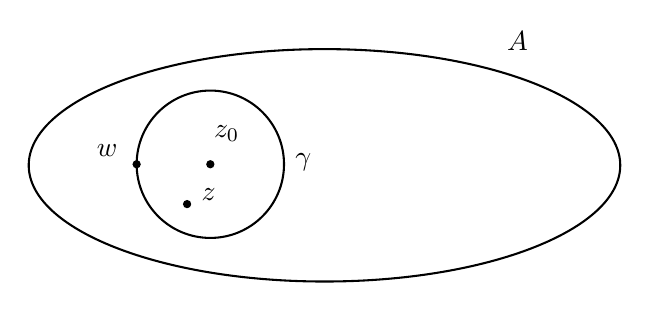
\begin{tikzpicture}[x=0.75pt,y=0.75pt,yscale=-1,xscale=1]
%uncomment if require: \path (0,136); %set diagram left start at 0, and has height of 136

%Shape: Ellipse [id:dp7479505317469046] 
\draw   (159,71.02) .. controls (159,40.1) and (222.8,15.03) .. (301.5,15.03) .. controls (380.2,15.03) and (444,40.1) .. (444,71.02) .. controls (444,101.93) and (380.2,127) .. (301.5,127) .. controls (222.8,127) and (159,101.93) .. (159,71.02) -- cycle ;
%Shape: Circle [id:dp8263143669411064] 
\draw   (211,70.5) .. controls (211,50.89) and (226.89,35) .. (246.5,35) .. controls (266.11,35) and (282,50.89) .. (282,70.5) .. controls (282,90.11) and (266.11,106) .. (246.5,106) .. controls (226.89,106) and (211,90.11) .. (211,70.5) -- cycle ;
%Shape: Circle [id:dp22698676265510276] 
\draw  [draw opacity=0][fill={rgb, 255:red, 0; green, 0; blue, 0 }  ,fill opacity=1 ] (244.5,70.5) .. controls (244.5,69.4) and (245.4,68.5) .. (246.5,68.5) .. controls (247.6,68.5) and (248.5,69.4) .. (248.5,70.5) .. controls (248.5,71.6) and (247.6,72.5) .. (246.5,72.5) .. controls (245.4,72.5) and (244.5,71.6) .. (244.5,70.5) -- cycle ;
%Shape: Circle [id:dp17321185166040398] 
\draw  [draw opacity=0][fill={rgb, 255:red, 0; green, 0; blue, 0 }  ,fill opacity=1 ] (233.3,89.7) .. controls (233.3,88.6) and (234.2,87.7) .. (235.3,87.7) .. controls (236.4,87.7) and (237.3,88.6) .. (237.3,89.7) .. controls (237.3,90.8) and (236.4,91.7) .. (235.3,91.7) .. controls (234.2,91.7) and (233.3,90.8) .. (233.3,89.7) -- cycle ;
%Shape: Circle [id:dp9508082191122853] 
\draw  [draw opacity=0][fill={rgb, 255:red, 0; green, 0; blue, 0 }  ,fill opacity=1 ] (209,70.5) .. controls (209,69.4) and (209.9,68.5) .. (211,68.5) .. controls (212.1,68.5) and (213,69.4) .. (213,70.5) .. controls (213,71.6) and (212.1,72.5) .. (211,72.5) .. controls (209.9,72.5) and (209,71.6) .. (209,70.5) -- cycle ;

% Text Node
\draw (190.4,59.6) node [anchor=north west][inner sep=0.75pt]    {$w$};
% Text Node
\draw (240.8,80.8) node [anchor=north west][inner sep=0.75pt]    {$z$};
% Text Node
\draw (246.8,50.4) node [anchor=north west][inner sep=0.75pt]    {$z_{0}$};
% Text Node
\draw (388,5.2) node [anchor=north west][inner sep=0.75pt]    {$A$};
% Text Node
\draw (286,64) node [anchor=north west][inner sep=0.75pt]    {$\gamma $};


\end{tikzpicture}
	
\end{figure}
\FloatBarrier



Sostituiamo nella formula di Cauchy
\begin{align*}
f( z) & =\frac{1}{2\pi i}\int _{\gamma } f( w)\sum ^{\infty }_{n=0}\frac{( z-z_{0})^{n}}{( w-z_{0})^{n+1}} dw\\
 & =\sum ^{\infty }_{n=0}( z-z_{0})^{n}\underbrace{\frac{1}{2\pi i}\int _{\gamma }\frac{f( w)}{( w-z_{0})^{n+1}} dw}_{a_{n}} =\sum ^{\infty }_{n=0} a_{n}( z-z_{0})^{n}
\end{align*}
Si noti che la regione considerata, come si vede in figura, è quindi una palla centrata in $z_{0}$.

Si ottiene anche la \textbf{formula per derivate}
\begin{gather*}
f^{(n)}( z_{0}) =\frac{n!}{2\pi i}\int _{\gamma }\frac{f(w)}{( w-z_{0})^{n+1}} dw\\
\qed 
\end{gather*}
\section{Serie di Laurent}

Vi sono dei punti particolari in certe funzioni dove non c'è convergenza della serie, ad esempio in $f( z) =\frac{1}{1-z}$ il punto $1$ è critico, e la serie geometrica associata non converge in tale punto (e di conseguenza nel disco). Queste "ostruzioni" sono di vario tipo e vengono opportunamente classificate.

Per risolvere il problema si introduce la Serie di Laurent, una nuova espansione su una corona circolare $A$ (quindi \textit{non} semplicemente connessa) centrata nel punto stesso che compromette l'espansione in serie di Taylor. Il teorema inoltre non richiede che la funzione $f$ sia olomorfa su tutto il dominio ma esclusivamente sulla corona circolare $A$.
\begin{theorem}
[Serie di Laurent] Sia $f\in H( A)$, $A=\{z\in \mathbb{C} :r< | z-z_{0}| < R\}$, $\gamma $ una curva regolare semplice chiusa in $A$ che concateni $z_{0}$. Allora
\begin{equation*}
\boxed{\forall z\in A,\ \ f( z) =\sum\limits ^{\infty }_{n=-\infty } a_{n}( z-z_{0})^{n} \ \ \ \ a_{n} =\frac{1}{2\pi i}\int _{\gamma }\frac{f( w)}{( w-z_{0})^{n+1}} dw}
\end{equation*}
\end{theorem}
Si noti che la curva è \textit{qualsiasi} purché concatenata con $z_{0}$; ciò deriva dal fatto che la funzione è olomorfa nel dominio dove si esegue l'integrazione, e pertanto l'integrale non varia per deformazione continua.

Il teorema di Laurent è pertanto una generalizzazione del teorema di Weierstrass, in cui si include anche una somma sui \textbf{termini negativi}. Sono proprio le potenze negative, infatti, a dare informazioni sul comportamento delle singolarità.

\textit{Dimostrazione.}

Tutto si basa sul \textit{fare un giro attorno al punto}



\begin{figure}[htpb]
	\centering
\tikzset{every picture/.style={line width=0.75pt}} %set default line width to 0.75pt        

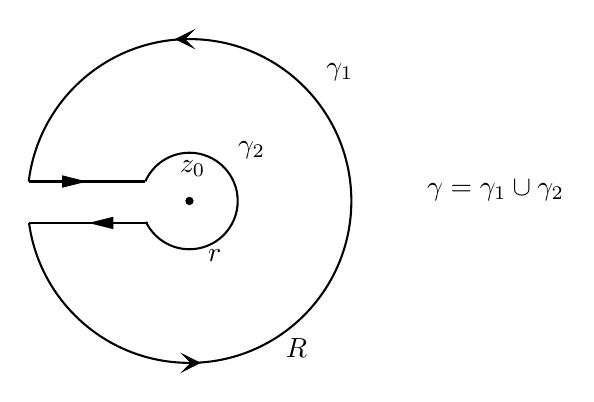
\begin{tikzpicture}[x=0.75pt,y=0.75pt,yscale=-1,xscale=1]
%uncomment if require: \path (0,184); %set diagram left start at 0, and has height of 184

%Shape: Arc [id:dp509954749685253] 
\draw  [draw opacity=0] (181.56,83.63) .. controls (186.19,44.97) and (219.09,15) .. (259,15) .. controls (302.08,15) and (337,49.92) .. (337,93) .. controls (337,136.08) and (302.08,171) .. (259,171) .. controls (219.52,171) and (186.89,141.66) .. (181.71,103.6) -- (259,93) -- cycle ; \draw   (181.56,83.63) .. controls (186.19,44.97) and (219.09,15) .. (259,15) .. controls (302.08,15) and (337,49.92) .. (337,93) .. controls (337,136.08) and (302.08,171) .. (259,171) .. controls (219.52,171) and (186.89,141.66) .. (181.71,103.6) ;
%Shape: Arc [id:dp39536995790567286] 
\draw  [draw opacity=0] (237.74,83.57) .. controls (241.36,75.43) and (249.52,69.75) .. (259,69.75) .. controls (271.84,69.75) and (282.25,80.16) .. (282.25,93) .. controls (282.25,105.84) and (271.84,116.25) .. (259,116.25) .. controls (249.77,116.25) and (241.79,110.87) .. (238.04,103.07) -- (259,93) -- cycle ; \draw   (237.74,83.57) .. controls (241.36,75.43) and (249.52,69.75) .. (259,69.75) .. controls (271.84,69.75) and (282.25,80.16) .. (282.25,93) .. controls (282.25,105.84) and (271.84,116.25) .. (259,116.25) .. controls (249.77,116.25) and (241.79,110.87) .. (238.04,103.07) ;
%Straight Lines [id:da39785143879926865] 
\draw    (181.71,103.6) -- (239,103.6) ;
\draw [shift={(210.36,103.6)}, rotate = 0] [fill={rgb, 255:red, 0; green, 0; blue, 0 }  ][line width=0.08]  [draw opacity=0] (12,-3) -- (0,0) -- (12,3) -- cycle    ;
%Straight Lines [id:da7721203931176552] 
\draw    (237.74,83.63) -- (181.56,83.63) ;
\draw [shift={(209.65,83.63)}, rotate = 180] [fill={rgb, 255:red, 0; green, 0; blue, 0 }  ][line width=0.08]  [draw opacity=0] (12,-3) -- (0,0) -- (12,3) -- cycle    ;
\draw  [draw opacity=0][fill={rgb, 255:red, 0; green, 0; blue, 0 }  ,fill opacity=1 ] (254.5,166) -- (264.5,171) -- (254.5,176) -- (259.5,171) -- cycle ;
\draw  [draw opacity=0][fill={rgb, 255:red, 0; green, 0; blue, 0 }  ,fill opacity=1 ] (262,20) -- (252,15) -- (262,10) -- (257,15) -- cycle ;
%Shape: Circle [id:dp12847517277803466] 
\draw  [draw opacity=0][fill={rgb, 255:red, 0; green, 0; blue, 0 }  ,fill opacity=1 ] (257,93) .. controls (257,91.9) and (257.9,91) .. (259,91) .. controls (260.1,91) and (261,91.9) .. (261,93) .. controls (261,94.1) and (260.1,95) .. (259,95) .. controls (257.9,95) and (257,94.1) .. (257,93) -- cycle ;

% Text Node
\draw (253,71.9) node [anchor=north west][inner sep=0.75pt]    {$z_{0}$};
% Text Node
\draw (266.5,114.9) node [anchor=north west][inner sep=0.75pt]    {$r$};
% Text Node
\draw (304,157.9) node [anchor=north west][inner sep=0.75pt]    {$R$};
% Text Node
\draw (323.5,25.4) node [anchor=north west][inner sep=0.75pt]    {$\gamma _{1}$};
% Text Node
\draw (281,62.9) node [anchor=north west][inner sep=0.75pt]    {$\gamma _{2}$};
% Text Node
\draw (372,81.4) node [anchor=north west][inner sep=0.75pt]    {$\gamma =\gamma _{1} \cup \gamma _{2}$};


\end{tikzpicture}
	
\end{figure}
\FloatBarrier



L'insieme \textit{pacman} è effettivamente semplicemente connesso, e lì la funzione è olomorfa, allora
\begin{equation*}
\int _{\gamma } f( z) dz=0=\int _{\gamma _{1}} f( z) dz-\int _{\gamma _{2}} f( z) dz
\end{equation*}
i termini paralleli si cancellano. Consideriamo un $z$ nella corona $A$
\begin{equation*}
f( z) =\frac{1}{2\pi i}\int _{\gamma }\frac{f( w)}{w-z} dw=\underbrace{\frac{1}{2\pi i}\int _{\gamma _{1}}\frac{f( w)}{w-z} dw}_{A}\underbrace{-\frac{1}{2\pi i}\int _{\gamma _{2}}\frac{f( w)}{w-z} dw}_{B}
\end{equation*}
Analizziamo i termini.

Termine $A$
\begin{gather*}
\frac{1}{w-z} =\frac{1}{w-z_{0} -( z-z_{0})} =\frac{1}{w-z_{0}}\frac{1}{1-\frac{z-z_{0}}{w-z_{0}}} =\sum\limits ^{\infty }_{n=0}\frac{( z-z_{0})^{n}}{( w-z_{0})^{n+1}}\\
\Rightarrow \ \ A=\frac{1}{2\pi i}\int _{\gamma _{1}} f( w)\sum\limits ^{\infty }_{n=0}\frac{( z-z_{0})^{n}}{( w-z_{0})^{n+1}} dw=\sum\limits ^{\infty }_{n=0} a_{n}( z-z_{0})^{n}
\end{gather*}
Termine $B$, quello \textit{sospetto} che non c'era nel caso di Weierstrass
\begin{align*}
\frac{-1}{w-z} & =\frac{-1}{w-z_{0} -( z-z_{0})} =\frac{1}{z-z_{0}}\frac{1}{1-\frac{w-z_{0}}{z-z_{0}}} =\sum\limits ^{\infty }_{n=0}\frac{( w-z_{0})^{n}}{( z-z_{0})^{n+1}}\\
 & =\sum\limits ^{\infty }_{n=1}\frac{( w-z_{0})^{n-1}}{( z-z_{0})^{n}} =\sum\limits ^{-\infty }_{n=-1}\frac{( z-z_{0})^{n}}{( w-z_{0})^{n+1}}
\end{align*}
Sostituendo tale quantità in $B$ si ottiene la tesi.
\begin{equation*}
\qed 
\end{equation*}
\textit{Esempio.}
\begin{equation*}
f( z) =\frac{\sin z}{z} =\frac{1}{\cancel{z}}\sum\limits ^{\infty }_{n=0}\frac{( -1)^{n} z^{2n\cancel{+1}}}{( 2n+1) !} =\sum\limits ^{\infty }_{n=0}\frac{( -1)^{n} z^{2n}}{( 2n+1) !}
\end{equation*}
Abbiamo potuto eliminare la singolarità!
\subsection{Classificazione delle singolarità}
\begin{definition}
[Punto singolare] Un punto $z_{0}$ si dice \textbf{singolare} (o critico) per una funzione $f( z)$ se non può essere incluso in nessun disco di convergenza della serie di potenze.
\end{definition}
Classifichiamo i punti singolari in base ai coefficienti $a_{n} \neq 0,n< 0$
\begin{itemize}
\item se non ce n'è \textit{nessuno:} \textbf{singolarità eliminabile} (esiste un prolungamento continuo)
\item se sono \textit{finiti:} \textbf{polo}
\begin{itemize}
\item definiamo inoltre l'\textbf{ordine} di un polo come l'indice $n >0$ dei coefficienti $a_{-n} \neq 0$ tale che $a_{m} =0,\forall m< -n$. Ovvero stiamo prendendo il più piccolo coefficiente non nullo.
\end{itemize}
\item se sono \textit{infiniti:} \textbf{singolarità essenziale}
\end{itemize}

\textit{Esempio.}
\begin{equation*}
z_{0} =1,\ \ f( z) =\frac{1}{z-1} =\sum\limits ^{\infty }_{n=-\infty } a_{n}( z-1)^{n} \ \ \ \ a_{n} =\begin{cases}
0, & n\neq -1\\
1, & n=-1
\end{cases}
\end{equation*}
in questo caso $z_{0}$ è un polo.

\textit{Esempio.}
\begin{equation*}
z_{0} =0,\ \ f( z) =\sin\left(\frac{1}{z}\right) =\sum\limits ^{\infty }_{n=0}\frac{\left(\frac{1}{z}\right)^{2n+1}( -1)^{n}}{( 2n+1) !} =\sum\limits ^{-\infty }_{n=0}\frac{z^{2n-1}( -1)^{n}}{( 1-2n) !}
\end{equation*}
in questo caso $z_{0}$ è una singolarità essenziale.
\begin{definition}
[Punto singolare isolato] Un punto singolare $z_{0}$ per $f( z)$ si dice \textbf{isolato} esiste un intorno che non contiene punti critici per $f$.
\end{definition}
In $\mathbb{C}$ non ha senso parlare di $\pm \infty $, essendoci infinite direzioni, tuttavia è utile considerare tutti i punti infinitamente distanti \textit{come un unico punto all'infinito}, più nello specifico vale la seguente definizione.
\begin{definition}
[Punto singolare all'infinito] Il punto all'infinito $z_{\infty }$ è singolare per $f( z)$ se $z_{0} =0$ è singolare per $f\left(\frac{1}{z}\right)$.
\end{definition}
\textit{Esempio.}

La funzione $f( z) =e^{z}$ ha singolarità isolata all'infinito, mentre $g( z) =\frac{1}{\sin z}$ ha punto all'infinito non isolato.


\begin{theorem}
[Caratterizzazione dei poli] Sia $z_{0} \neq \infty $ un punto singolare isolato per $f$. Allora le seguenti affermazioni sono equivalenti:
\begin{enumerate}
\item $f$ ha un polo di ordine $n$ in $z_{0}$;
\item $g(z)=( z-z_{0})^{n} f(z)$ ha una singolarità eliminabile in $z_{0}$ e inoltre $\lim _{z\rightarrow z_{0}} g(z)\neq 0$;
\item è rispettata la seguente relazione tra ordini di grandezza:

\begin{equation*}
|f(z)|\asymp \frac{1}{| z-z_{0}| ^{n}}
\end{equation*}
\item $\varphi (z)=\frac{1}{f(z)}$ ha in $z_{0}$ uno zero di ordine $n$.
\end{enumerate}
\end{theorem}

\begin{theorem}
[Caratterizzazione delle singolarità] Valgono le seguenti affermazioni, con $z_{0}$ punto singolare isolato per $f$ :
\begin{enumerate}
\item $\lim _{z\rightarrow z_{0}} f(z)=\infty \Leftrightarrow z_{0}$ è un polo.
\item $\lim _{z\rightarrow z_{0}} f(z)$ esiste finito $\Leftrightarrow z_{0}$ è una singolarità eliminabile.
\item $\lim _{z\rightarrow z_{0}} f(z)$ non esiste $\Leftrightarrow z_{0}$ è una singolarità essenziale.
\end{enumerate}
\end{theorem}
\begin{theorem}
[Caratterizzazione delle singolarità essenziali] Sia $z_{0}$ una singolarità essenziale isolata per $f(z)$. Allora la funzione $\frac{1}{f(z)}$ ha in $z_{0}$ una singolarità essenziale oppure un punto di accumulazione di poli.
\end{theorem}
In generale si può sempre studiare la serie di Laurent centrata nel punto, ma ciò può risultare complicato e lungo da fare, specialmente se le singolarità sono molte.
\section{Teorema dei residui}

Il coefficiente $a_{-1}$ della serie di Laurent centrata in $z_{0}$ è molto importante e prende il nome di \textbf{residuo integrale}
\begin{equation*}
a_{n} =\frac{1}{2\pi i}\int _{\gamma }\frac{f( w)}{( w-z_{0})^{n+1}} dw\ \ \Rightarrow \ \ \mathrm{Res}( f,z_{0}) =a_{-1} =\frac{1}{2\pi i}\int _{\gamma } f( w) dw
\end{equation*}
Il seguente teorema semplifica tantissimi calcoli di integrali, anche reali.
\begin{theorem}
[dei Residui] Sia $A\subset \mathbb{C}$ aperto, $f\in H( A\setminus \{z_{1} ,\dotsc ,z_{n}\} \cap C^{0}(\overline{A} \setminus \{z_{1} ,\dotsc ,z_{n}\})$. Allora
\begin{equation*}
\boxed{\int _{\gamma } f( z) dz=2\pi i\cdotp \sum\limits ^{n}_{j=1}\mathrm{Res}( f,z_{j})}
\end{equation*}
\end{theorem}
\begin{definition}
Se consideriamo una $\gamma $ chiusa che contiene tutte le singolarità di $f( z)$ al finito, e $f\in H(| z|  >R)$, se consideriamo lo sviluppo di $f$ in un intorno dell'infinito, allora definiamo il \textbf{residuo all'infinito}
\begin{equation*}
\mathrm{Res}( f,\infty ) :=-a_{-1} =\frac{1}{2\pi i}\int _{-\gamma } f( w) dw
\end{equation*}
\end{definition}
\begin{theorem}
Se abbiamo un numero finito di singolarità, la somma di tutte, sia al finito che all'infinito, vale zero.
\begin{equation*}
\sum\limits ^{n}_{j=1}\mathrm{Res}( f,z_{j}) +\mathrm{Res}( f,\infty ) =0
\end{equation*}
\end{theorem}
\subsection{Come calcolare i residui}

Se $z_{0} \neq \infty $
\begin{itemize}
\item se è eliminabile allora $\mathrm{Res}( f,z_{0}) =0$
\item se è polo di ordine $n$ allora $\mathrm{Res}( f,z_{0}) =\lim\limits _{z\rightarrow z_{0}}\frac{d^{n-1}}{dz^{n-1}}\frac{( z-z_{0})^{n}}{n!} f( z)$
\item se è polo di ordine $1$ allora $\mathrm{Res}\left(\frac{f}{g} ,z_{0}\right) =\lim\limits _{z\rightarrow z_{0}}\frac{f( z)}{g'( z)}$
\item vale L'Hopital $\lim\limits _{z\rightarrow z_{0}}\frac{f(z)}{g(z)} =\lim\limits _{z\rightarrow z_{0}}\frac{f'(z)}{g'(z)}$
\end{itemize}

Se $z_{0} =\infty $
\begin{itemize}
\item $\mathrm{Res}( f,\infty ) =\mathrm{Res}\left( -\frac{1}{z^{2}} f\left(\frac{1}{z}\right) ,0\right)$
\item se è zero di ordine $1$ allora $\mathrm{Res}( f,\infty ) =-\lim\limits _{z\rightarrow \infty } zf( z)$
\item se è zero di ordine $\geqslant 2$ allora $\mathrm{Res}( f,\infty ) =0$
\end{itemize}
\section{Lemmi di Jordan}

Consideriamo un generico arco di circonferenza:
\begin{equation*}
C_{R}( \vartheta _{1} ,\vartheta _{2}) =\left\{z\in \mathbb{C} :z=Re^{i\vartheta } ,\vartheta \in [ \vartheta _{1} ,\vartheta _{2}]\right\}
\end{equation*}
\begin{theorem}
Sia $f(z)$ continua su $C_{R}$. Allora:
\begin{equation*}
\left| \int _{C_{R}} f(z)dz\right| \leqslant R( \vartheta _{2} -\vartheta _{1})\max_{|z\in C_{R}}| f(z)| 
\end{equation*}
dove $R( \vartheta _{2} -\vartheta _{1})$ non è altro che la lunghezza dell'arco.
\end{theorem}
\begin{theorem}
[Lemma di Jordan al cerchio grande] Sia $K >0$ e sia $f(z)$ continua per $|z| >K$. Se $\exists \alpha  >1,c >0$ tali che $|f(z)|\leqslant \frac{c}{|z|^{\alpha }} ,\ \forall z:|z| >K,$ allora:
\begin{equation*}
\lim _{R\rightarrow \infty }\int _{C_{R}( \vartheta _{1} ,\vartheta _{2})} f(z)dz=0\ \ \forall \vartheta _{1} ,\vartheta _{2}
\end{equation*}
\end{theorem}
\textit{Dimostrazione.}
\begin{equation*}
\left| \int f( z) dz\right| \leqslant R( \vartheta _{2} -\vartheta _{1})\frac{c}{|z|^{\alpha }} =R( \vartheta _{2} -\vartheta _{1})\frac{c}{R^{\alpha }}\xrightarrow[\alpha  >1]{R\rightarrow \infty } 0
\end{equation*}
\begin{theorem}
[Lemma di Jordan al cerchio piccolo] Con analoghe ipotesi ma con $\alpha < 1$
\begin{equation*}
\lim _{R\rightarrow 0}\int _{C_{R}( \vartheta _{1} ,\vartheta _{2})} f(z)dz=0\ \ \forall \vartheta _{1} ,\vartheta _{2}
\end{equation*}
\end{theorem}
Tuttavia $f$ può andare a zero anche più lentamente per ottenere dei risultati interessanti
\begin{theorem}
[Lemmi di Jordan] Sia $f(z)$ continua per $|z| >K.$ Siano inoltre $\vartheta _{1} ,\vartheta _{2} \in [0,2\pi ]$ e $a >0,$tali che:
\begin{equation*}
\lim _{R\rightarrow \infty }\sup _{z\in C_{R}}| f( z)| =0
\end{equation*}
Allora:
\begin{enumerate}
\item se $\vartheta _{1} =0$ e $\vartheta _{2} =\pi $

\begin{equation*}
\lim _{R\rightarrow \infty }\int _{C_{R} (0,\pi )} e^{iaz} f(z)dz=0
\end{equation*}
\item se $\vartheta _{1} =\pi $ e $\vartheta _{2} =2\pi $,

\begin{equation*}
\lim _{R\rightarrow \infty }\int _{C_{R} (\pi ,2\pi )} e^{-iaz} f(z)dz=0
\end{equation*}
\item se $\vartheta _{1} =-\frac{\pi }{2}$ e $\vartheta _{2} =\frac{\pi }{2}$,

\begin{equation*}
\lim _{R\rightarrow \infty }\int _{C_{R}\left( -\frac{\pi }{2} ,\frac{\pi }{2}\right)} e^{-az} f(z)dz=0
\end{equation*}
\item se $\vartheta _{1} =\frac{\pi }{2}$ e $\vartheta _{2} =\frac{3}{2} \pi $,

\begin{equation*}
\lim _{R\rightarrow \infty }\int _{C_{R}\left(\frac{\pi }{2} ,\frac{3}{2} \pi \right)} e^{az} f(z)dz=0
\end{equation*}
\end{enumerate}
\end{theorem}
\textit{Dimostrazione di }$( 1)$

Sia $z=Re^{i\vartheta }$, $\vartheta \in [ 0,\pi ]$, sostituiamo
\begin{equation*}
\int _{C_{R} (0,\pi )} e^{iaz} f(z)dz=\int ^{\pi }_{0} e^{iaRe^{i\vartheta }} f\left( Re^{i\vartheta }\right) iRe^{i\vartheta } d\vartheta 
\end{equation*}
Poniamo $M=\sup _{z\in C_{R}}| f( z)| $, per ipotesi $\lim _{R\rightarrow \infty } M=0$. Notiamo che
\begin{equation*}
e^{iaRe^{i\vartheta }} =e^{iaR[\cos \vartheta +i\sin \vartheta ]} =\underbrace{e^{iaR\cos \vartheta }}_{\text{modulo} \ 1} e^{-aR\sin \vartheta }
\end{equation*}
Maggioriamo
\begin{equation*}
\left| \int _{C_{R} (0,\pi )} e^{iaz} f(z)dz\right| \leqslant M\int ^{\pi }_{0}\left| e^{iaRe^{i\vartheta }} iRe^{i\vartheta }\right| d\vartheta =2MR\int ^{\pi /2}_{0} e^{-aR\sin \vartheta } d\vartheta =( *)
\end{equation*}
a questo punto possiamo minorare il seno con la retta che passa per $0$ e $( \pi /2,1)$
\begin{equation*}
\sin \vartheta \geqslant \frac{2\vartheta }{\pi }
\end{equation*}
Di conseguenza
\begin{equation*}
( *) \leqslant 2MR\int ^{\pi /2}_{0} e^{-aR\frac{2\vartheta }{\pi }} d\vartheta =\cancel{2} M\cancel{R}\left[\left( -\frac{\pi }{\cancel{2} a\cancel{R}}\right) e^{-aR\frac{2\vartheta }{\pi }}\right]^{\pi /2}_{0} =-\frac{\pi M}{a}\underbrace{\left[ e^{-aR} -1\right]}_{\in [ -1,0]} \leqslant \frac{\pi M}{a}
\end{equation*}
Per ipotesi $M\rightarrow 0$ e $a >0$, da cui la tesi.
\begin{equation*}
\qed 
\end{equation*}



\chapter{Spazi di Banach e Spazi di Hilbert}
\begin{definition}
[Norma] Sia $X$ uno spazio vettoriale. Si dice \textbf{norma} un'applicazione $\Vert \cdotp \Vert :X\rightarrow [ 0,+\infty )$ che verifica, $\forall \lambda \in \mathbb{R}$, $\forall x,y\in X$
\begin{itemize}
\item $\Vert x\Vert =0\Leftrightarrow x=0$
\item $\Vert \lambda x\Vert =| \lambda | \Vert x\Vert $
\item $\Vert x+y\Vert \leqslant \Vert x\Vert +\Vert y\Vert $
\end{itemize}
\end{definition}

\textit{Esempio.}

Dato $1\leqslant p< +\infty $, l'applicazione $\Vert \cdotp \Vert :\mathbb{R}^{n}\rightarrow [ 0,+\infty )$ definita da
\begin{equation*}
\Vert x\Vert _{p} =\left(| x_{1}| ^{p} +\dotsc +| x_{n}| ^{p}\right)^{1/p}
\end{equation*}
è la norma $p$.

\textit{Esempio.}

L'applicazione $\Vert \cdotp \Vert :\mathbb{R}^{n}\rightarrow [ 0,+\infty )$ definita da
\begin{equation*}
\Vert x\Vert _{\infty } =\max\{| x_{1}| ,\dotsc ,| x_{n}| \}
\end{equation*}
è la norma infinito.
\begin{definition}
[Spazio normato] Uno spazio vettoriale dotato di norma si dice \textbf{spazio normato}.
\end{definition}
\begin{definition}
[Metrica] La funzione $d:X\times X\rightarrow [ 0,+\infty )$ definita da $( u,v) =\Vert u-v\Vert $ è detta \textbf{metrica} indotta dalla norma, mentre la quantità $\Vert u-v\Vert $ è detta \textbf{distanza}.
\end{definition}
\begin{definition}
[Spazio metrico] Uno spazio vettoriale dotato di metrica si dice \textbf{spazio metrico}, quindi uno spazio normato è anche metrico.
\end{definition}
\begin{definition}
[Successione di Cauchy] Sia $V$ uno spazio normato. Una successione $x_{n}$ è di Cauchy se $\forall \varepsilon  >0$, $\exists N$ tale che $\forall n,m\geqslant N$ si ha $\Vert x_{n} -x_{m}\Vert < \varepsilon $. Ogni successione convergente è di Cauchy.
\end{definition}
\begin{definition}
[Spazio completo] Uno spazio metrico si dice \textbf{completo} se ogni successione di Cauchy è convergente.
\end{definition}
\begin{definition}
[Spazio di Banach] Uno spazio normato si dice di Banach se è completo.
\end{definition}
\begin{definition}
[Prodotto scalare] Il prodotto scalare è un'applicazione $( \cdotp ,\cdotp ) :X\times X\rightarrow \mathbb{C}$ tale che
\begin{itemize}
\item $( x,x) =0\Leftrightarrow x=0$
\item $( x,x) \geqslant 0,\forall x\in X$
\item $( x,y) =\overline{( y,x)}$
\item Vale la \textit{sesquilinearità}
\begin{itemize}
\item $( c_{1} x_{1} +c_{2} x_{2} ,y) =c_{1}( x_{1} ,y) +c_{2}( x_{2} ,y)$
\item $\overline{( y,c_{1} x_{1} +c_{2} x_{2})} =c_{1}\overline{( y,x_{1})} +c_{2}\overline{( y,x_{2})}$
\item $( y,c_{1} x_{1} +c_{2} x_{2}) =\overline{c_{1}}( y,x_{1}) +\overline{c_{2}}( y,x_{2})$
\end{itemize}
\end{itemize}
\end{definition}
\begin{definition}
[Spazio di Hilbert] Uno spazio vettoriale \textit{dotato di prodotto scalare} (che induce quindi una norma $\Vert x\Vert =\sqrt{( x,x)}$ e una distanza) \textit{e completo} rispetto a quella norma si dice \textbf{spazio di Hilbert}.
\end{definition}
\begin{definition}
Definiamo lo spazio delle successioni convergenti
\begin{equation*}
l^{2} =\left\{\{a_{n}\} \subset \mathbb{C} :\sum\limits ^{\infty }_{n=0}| a_{n}| ^{2} < +\infty \right\}
\end{equation*}
\end{definition}
\begin{definition}
[Spazio convesso] Dato uno spazio di Hilbert $H$, $K\subset H$, $K$ è \textbf{convesso} se $\forall x,y\in K,\forall \lambda \in [ 0,1]$ allora $\lambda x+( 1-\lambda ) y\in K$.
\end{definition}
\begin{theorem}
[di proiezione] Sia $H$ di Hilbert e $C\subset H$ convesso e chiuso. Sia $\overline{x} \notin C$, allora $\exists P\in C$ tale che
\begin{equation*}
\Vert \overline{x} -P\Vert \leqslant \Vert \overline{x} -x\Vert \ \ \forall x\in C
\end{equation*}
e
\begin{equation*}
(\overline{x} -P,x-p) \leqslant 0\ \ \forall x\in C
\end{equation*}
\end{theorem}


\begin{figure}[htpb]
	\centering
	\tikzset{every picture/.style={line width=0.75pt}} %set default line width to 0.75pt        

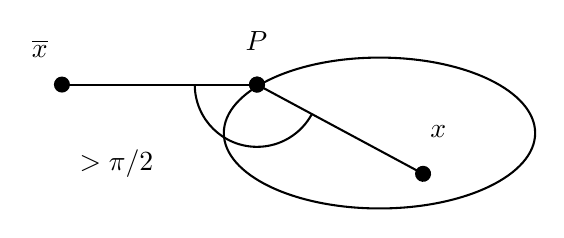
\begin{tikzpicture}[x=0.75pt,y=0.75pt,yscale=-1,xscale=1]
%uncomment if require: \path (0,106); %set diagram left start at 0, and has height of 106

%Shape: Ellipse [id:dp5649356596549697] 
\draw   (267,60.66) .. controls (267,40.58) and (300.58,24.31) .. (342,24.31) .. controls (383.42,24.31) and (417,40.58) .. (417,60.66) .. controls (417,80.73) and (383.42,97) .. (342,97) .. controls (300.58,97) and (267,80.73) .. (267,60.66) -- cycle ;
%Straight Lines [id:da02100518467366297] 
\draw    (283,37.31) -- (189,37.31) ;
\draw [shift={(189,37.31)}, rotate = 180] [color={rgb, 255:red, 0; green, 0; blue, 0 }  ][fill={rgb, 255:red, 0; green, 0; blue, 0 }  ][line width=0.75]      (0, 0) circle [x radius= 3.35, y radius= 3.35]   ;
\draw [shift={(283,37.31)}, rotate = 180] [color={rgb, 255:red, 0; green, 0; blue, 0 }  ][fill={rgb, 255:red, 0; green, 0; blue, 0 }  ][line width=0.75]      (0, 0) circle [x radius= 3.35, y radius= 3.35]   ;
%Straight Lines [id:da7214240046750127] 
\draw    (363,80.31) -- (283,37.31) ;
\draw [shift={(283,37.31)}, rotate = 208.26] [color={rgb, 255:red, 0; green, 0; blue, 0 }  ][fill={rgb, 255:red, 0; green, 0; blue, 0 }  ][line width=0.75]      (0, 0) circle [x radius= 3.35, y radius= 3.35]   ;
\draw [shift={(363,80.31)}, rotate = 208.26] [color={rgb, 255:red, 0; green, 0; blue, 0 }  ][fill={rgb, 255:red, 0; green, 0; blue, 0 }  ][line width=0.75]      (0, 0) circle [x radius= 3.35, y radius= 3.35]   ;
%Shape: Arc [id:dp82817523637768] 
\draw  [draw opacity=0] (309.33,51.7) .. controls (304.23,61.01) and (294.35,67.31) .. (283,67.31) .. controls (266.58,67.31) and (253.25,54.13) .. (253,37.77) -- (283,37.31) -- cycle ; \draw   (309.33,51.7) .. controls (304.23,61.01) and (294.35,67.31) .. (283,67.31) .. controls (266.58,67.31) and (253.25,54.13) .. (253,37.77) ;

% Text Node
\draw (173,14.4) node [anchor=north west][inner sep=0.75pt]    {$\overline{x}$};
% Text Node
\draw (276,10.4) node [anchor=north west][inner sep=0.75pt]    {$P$};
% Text Node
\draw (365,55.4) node [anchor=north west][inner sep=0.75pt]    {$x$};
% Text Node
\draw (196,67.4) node [anchor=north west][inner sep=0.75pt]    {$ >\pi /2$};


\end{tikzpicture}
\end{figure}
\FloatBarrier

Chiameremo $P_{C}\overline{x}$ la proiezione di $\overline{x}$ su $C$.

Consideriamo $M\subset H$ sottospazio chiuso (essenziale per includere anche il caso in cui $H$ ha dimensione infinita). Sia $\overline{x} \in M$, consideriamo il caso bidimensionale con $M$ che ha dimensione $1$, si può chiaramente scomporre
\begin{equation*}
\textcolor[rgb]{0.29,0.56,0.89}{\overline{x}} =\overline{x} -P_{M}\overline{x} +P_{M}\overline{x} =\textcolor[rgb]{0.49,0.83,0.13}{Q}\textcolor[rgb]{0.49,0.83,0.13}{_{M}}\textcolor[rgb]{0.49,0.83,0.13}{\overline{x}} +\textcolor[rgb]{0.82,0.01,0.11}{P}\textcolor[rgb]{0.82,0.01,0.11}{_{M}}\textcolor[rgb]{0.82,0.01,0.11}{\overline{x}}
\end{equation*}


\begin{figure}[htpb]
	\centering
	\tikzset{every picture/.style={line width=0.75pt}} %set default line width to 0.75pt        

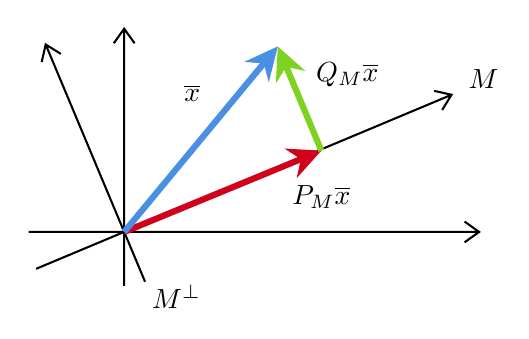
\begin{tikzpicture}[x=0.75pt,y=0.75pt,yscale=-1,xscale=1]
%uncomment if require: \path (0,184); %set diagram left start at 0, and has height of 184

%Shape: Axis 2D [id:dp7134109691601231] 
\draw  (198,127.91) -- (415,127.91)(244,30) -- (244,153.91) (408,122.91) -- (415,127.91) -- (408,132.91) (239,37) -- (244,30) -- (249,37)  ;
%Shape: Axis 2D [id:dp2976528104012621] 
\draw  (201.57,145.68) -- (401.72,61.83)(206.17,37.6) -- (254.05,151.89) (393.33,59.93) -- (401.72,61.83) -- (397.2,69.15) (204.26,45.99) -- (206.17,37.6) -- (213.49,42.13)  ;
%Straight Lines [id:da6603280695196603] 
\draw [color={rgb, 255:red, 208; green, 2; blue, 27 }  ,draw opacity=1 ][line width=2.25]    (244,127.91) -- (334.38,90.66) ;
\draw [shift={(339,88.75)}, rotate = 517.6] [fill={rgb, 255:red, 208; green, 2; blue, 27 }  ,fill opacity=1 ][line width=0.08]  [draw opacity=0] (16.07,-7.72) -- (0,0) -- (16.07,7.72) -- (10.67,0) -- cycle    ;
%Straight Lines [id:da12421560052711267] 
\draw [color={rgb, 255:red, 74; green, 144; blue, 226 }  ,draw opacity=1 ][line width=2.25]    (244,127.91) -- (314.81,42.38) ;
\draw [shift={(318,38.53)}, rotate = 489.62] [fill={rgb, 255:red, 74; green, 144; blue, 226 }  ,fill opacity=1 ][line width=0.08]  [draw opacity=0] (16.07,-7.72) -- (0,0) -- (16.07,7.72) -- (10.67,0) -- cycle    ;
%Straight Lines [id:da9584665613249306] 
\draw [color={rgb, 255:red, 126; green, 211; blue, 33 }  ,draw opacity=1 ][line width=2.25]    (339,88.75) -- (319.93,43.15) ;
\draw [shift={(318,38.53)}, rotate = 427.31] [fill={rgb, 255:red, 126; green, 211; blue, 33 }  ,fill opacity=1 ][line width=0.08]  [draw opacity=0] (16.07,-7.72) -- (0,0) -- (16.07,7.72) -- (10.67,0) -- cycle    ;

% Text Node
\draw (408.5,48.4) node [anchor=north west][inner sep=0.75pt]    {$M$};
% Text Node
\draw (256,151.9) node [anchor=north west][inner sep=0.75pt]    {$M^{\perp }$};
% Text Node
\draw (271.5,55.4) node [anchor=north west][inner sep=0.75pt]    {$\overline{x}$};
% Text Node
\draw (335,44.9) node [anchor=north west][inner sep=0.75pt]    {$Q_{M}\overline{x}$};
% Text Node
\draw (323.5,103.9) node [anchor=north west][inner sep=0.75pt]    {$P_{M}\overline{x}$};


\end{tikzpicture}
\end{figure}
\FloatBarrier

\begin{definition}
[Spazio ortogonale] Sia $H$ di Hilbert, sia $M\subset H$ un sottospazio chiuso. Chiamiamo spazio ortogonale a $M$ lo spazio
\begin{equation*}
M^{\perp } =\{x\in H:( x,y) =0,\forall y\in M\}
\end{equation*}
\end{definition}
Uno spazio di Hilbert è la più naturale estensione di uno spazio euclideo a dimensione infinita.
\begin{theorem}
[di proiezione] Sia $H$ di Hilbert, sia $M\subset H$ un sottospazio \textbf{chiuso proprio}. Allora
\begin{enumerate}
\item $\forall x\in H,\exists !$ decomposizione in $\mathbb{R}^{n}$ generica\begin{equation*}
x=P_{x} +Q_{x}
\end{equation*}
tale che $P_{x} \in M$, $Q_{x} \in M^{\perp }$.
\item detti $P=P_{M}$ e $Q=P_{M^{\perp }}$ le proiezioni di un certo punto rispettivamente su $M$ e $M^{\perp }$, allora\begin{gather*}
\Vert P_{x} -x\Vert \leqslant \Vert y-x\Vert \ \ \forall y\in M\\
\Vert Q_{x} -x\Vert \leqslant \Vert y-x\Vert \ \ \forall y\in M^{\perp }
\end{gather*}
\item le applicazioni $P:H\rightarrow M$ e $Q:H\rightarrow M^{\perp }$ sono lineari
\item vale Pitagora generalizzato\begin{equation*}
\Vert x\Vert ^{2} =\Vert P\Vert ^{2} +\Vert Q\Vert ^{2}
\end{equation*}
\end{enumerate}
\end{theorem}

Il teorema ha come corollario del quarto punto che proiettando due punti non li possiamo allontanare più di quanto non lo erano
\begin{equation*}
\Vert P_{x} -P_{y}\Vert \leqslant \Vert x-y\Vert \ \ \forall x,y
\end{equation*}
\begin{oss}
I casi banali sono
\begin{gather*}
x\in M\Rightarrow P=x,Q=0\\
x\in M^{\perp } \Rightarrow P=0,Q=x
\end{gather*}
\end{oss}
\begin{theorem}
[Disuguaglianza di Schwarz]
\begin{equation*}
| ( x,y)| \leqslant \Vert x\Vert \Vert y\Vert \ \ \forall x,y\in H
\end{equation*}
\end{theorem}
\begin{theorem}
[Identità del parallelogramma] La somma dei quadrati sulle diagonali è uguale alla somma dei quadrati su tutti i lati
\begin{equation*}
\Vert x+y\Vert ^{2} +\Vert x-y\Vert ^{2} =2\left(\Vert x\Vert ^{2} +\Vert y\Vert ^{2}\right)
\end{equation*}
\end{theorem}
\begin{definition}
[Spazio separabile] Uno spazio normato $X$ si dice separabile se $\exists Y\subset X$, $Y$ numerabile e tale che $\overline{Y} =X$.
\end{definition}
In uno spazio separabile si ha che $\forall x\in X,\exists \{y_{n}\} \subset Y$ tale che $y_{n}\rightarrow x$, cioè nel senso della norma $\Vert y_{n} -x\Vert \rightarrow 0$. Si dice che $Y$ è denso in $X$, ovvero possiamo sempre trovare una successione approssimante.
\begin{definition}
[Base hilbertiana] Sia $H$ di Hilbert a dimensione infinita. Un insieme di vettori $\{e_{k}\} \subset H$ tali che $( e_{j} ,e_{k}) =\delta _{jk}$ si dice \textbf{base hilbertiana} se $\forall x\in H,\exists \{\lambda _{n}\} \subset \mathbb{C}$ tale che $x=\sum ^{\infty }_{n=1} \lambda _{n} e_{n}$.
\end{definition}
\begin{oss}
Non essendo finita, non è una base nel senso dell'algebra lineare, ma è la cosa più vicina in dimensione infinita.
\end{oss}
\begin{oss}
È l'equivalente di una base ortonormale.
\end{oss}
\begin{oss}
Se $n=\mathrm{dim}( V) < \infty $, $\{e_{1} ,\dotsc ,e_{n}\}$, $( e_{j} ,e_{k}) =\delta _{jk}$, allora $\forall v\in V\Rightarrow v=\sum ^{n}_{k=1} \lambda _{k} e_{k}$.
\end{oss}
\begin{oss}
Dire
\begin{equation*}
x=\sum ^{\infty }_{n=1} \lambda _{n} e_{n} \ \ \text{è equivalente a dire} \ \ \lim\limits _{n\rightarrow +\infty }\left\Vert x-\sum ^{n}_{k=1} \lambda _{k} e_{k}\right\Vert =0
\end{equation*}
usando la norma indotta dal prodotto scalare.
\end{oss}
\begin{theorem}
Ogni spazio di Hilbert separabile ammette base Hilbertiana.
\end{theorem}
\begin{oss}
Il concetto di separabilità è un concetto abbastanza debole con poche richieste, soddisfatte nella stragrande maggioranza dei casi.
\end{oss}
\begin{theorem}
Sia $H$ separabile e sia $\{e_{n}\}$ una base hilbertiana. Allora $\forall x\in H$, $x$ si scrive come \textbf{serie di Fourier generalizzata}
\begin{equation*}
x=\sum ^{\infty }_{n=1}( x,e_{n}) e_{n}
\end{equation*}
dove pertanto definiamo i \textbf{coefficienti di Fourier}
\begin{equation*}
\lambda _{n} =( x,e_{n})
\end{equation*}
inoltre vale l'\textbf{identità di Parseval}
\begin{equation*}
\Vert x\Vert ^{2} =\sum\limits ^{\infty }_{n=1}| ( x,e_{n})| ^{2}
\end{equation*}
\end{theorem}
\textit{Semi-dimostrazione.}

Ammettendo base hilbertiana, esistono $\lambda _{n}$ tali che
\begin{equation*}
x=\sum ^{\infty }_{n=1} \lambda _{n} e_{n}
\end{equation*}
moltiplichiamo \textit{a destra} scalarmente per un generico $e_{k}$
\begin{equation*}
( x,e_{k}) =\left(\sum ^{\infty }_{n=1} \lambda _{n} e_{n} ,e_{k}\right) =\sum ^{\infty }_{n=1} \lambda _{n}( e_{n} ,e_{k})\overset{\delta _{nk}}{=} \lambda _{k}
\end{equation*}
\begin{oss}
È una semidimostrazione in quanto la linearità non vale per la serie che va a $\infty $, bisognerebbe passare al limite ma ci accontentiamo.
\end{oss}
Mostriamo ora Parseval
\begin{gather*}
\begin{aligned}
\Vert x\Vert ^{2} & =( x,x) =\left(\sum ^{\infty }_{n=1}( x,e_{n}) e_{n} ,\sum ^{\infty }_{k=1}( x,e_{k}) e_{k}\right)\\
 & =\sum\limits ^{\infty }_{n,k=1}( x,e_{n})\overline{( x,e_{k})}( e_{n} ,e_{k}) =\sum\limits ^{\infty }_{n=1}| ( x,e_{n})| ^{2}
\end{aligned}\\
\qed 
\end{gather*}
\begin{theorem}
Sia $H$ di Hilbert separabile. Allora $H$ è isomorfo a $l^{2}$. In particolare $\exists L:H\rightarrow l^{2}$, lineare, biiettiva ed isometria.
\end{theorem}
\begin{oss}
Quindi tutti gli spazi di Hilbert sono isomorfi tra di loro.
\end{oss}
\textit{Dimostrazione.}

Essendo separabile esiste una BH\footnote{Base Hilbertiana.} $\{e_{n}\}$.
\begin{equation*}
\forall x\in H\ \ \exists \lambda _{n} =( x,e_{n}) \ \ x=\sum ^{\infty }_{n=1} \lambda _{n} e_{n}
\end{equation*}
La successione dei coefficienti è contenuta in $l^{2}$
\begin{equation*}
\lambda =\{\lambda _{n}\} \subset l^{2}
\end{equation*}
grazie all'identità di Parseval
\begin{equation*}
\Vert x\Vert ^{2} =\sum\limits ^{\infty }_{n=1}| \lambda _{n}| ^{2}
\end{equation*}
Questa successione è anche unica, quindi la mappa è ben definita.
\begin{itemize}
\item \textit{Linearità.}\begin{equation*}
\lambda _{n} =( \alpha x+\beta y,e_{n}) =\alpha ( x,e_{n}) +\beta ( y,e_{n}) =\alpha \mu _{n} +\beta \nu _{n}
\end{equation*}
\item \textit{Isometria.}

Per Parseval\begin{equation*}
\Vert x\Vert ^{2}_{H} =\sum ^{\infty }_{n=1}| \lambda _{n}| ^{2} =\Vert \lambda \Vert ^{2}_{l^{2}}
\end{equation*}
\item \textit{Iniettività.}

Isometria significa che $\Vert L( x)\Vert =\Vert x\Vert $, grazie a questo possiamo dire che\footnote{Un'applicazione \textit{lineare} tra spazi di dimensione infinita \textit{può non essere continua}, ma se è isometria lo è di sicuro.}\begin{equation*}
L( x) =L( y) \ \ \Rightarrow \ \ \Vert L( x) -L( y)\Vert =0\ \ \Rightarrow \ \ \Vert x-y\Vert =0\ \ \Rightarrow \ \ x=y
\end{equation*}
\item \textit{Suriettività.}

Data $\lambda \subset l^{2} \mapsto x\in H,\lambda =L( x)$ dobbiamo costruire $x$ avendo $\lambda $, lo facciamo chiedendoci se converge\begin{equation*}
x=\sum ^{\infty }_{n=1} \lambda _{n} e_{n}
\end{equation*}

Usiamo la \textbf{completezza} dello spazio\begin{equation*}
\lambda \subset l^{2} \ \ \Rightarrow \ \ \sum\limits ^{\infty }_{n=1}| \lambda _{n}| ^{2} < +\infty \ \ \Rightarrow \ \ \mu _{k} =\sum\limits ^{k}_{n=1}| \lambda _{n}| ^{2} \ \ \text{è di Cauchy}
\end{equation*}

da cui possiamo considerare\begin{equation*}
x_{k} =\sum ^{k}_{n=1} \lambda _{n} e_{n}
\end{equation*}

e dimostrare che

\begin{gather*}
\Vert x_{k} -x_{l}\Vert =\left\Vert \sum\limits ^{k}_{n=l+1} \lambda _{n} e_{n}\right\Vert =\sum\limits ^{k}_{n=l+1}| \lambda _{n}| ^{2} =\mu _{k} -\mu _{l}\\
\Rightarrow \ \ x_{k} =\sum ^{k}_{n=1} \lambda _{n} e_{n} \ \ \text{è di Cauchy} \ \ \Rightarrow \ \ \text{converge per completezza.}\\
\qed 
\end{gather*}
\end{itemize}
\section{Integrale di Lebesgue}

Consideriamo un \textbf{plurirettangolo}
\begin{equation*}
P\subset \mathbb{R}^{n} ,\ \ P=[ a_{1} ,b_{1}] \times \dotsc \times [ a_{n} ,b_{n}]
\end{equation*}
la sua \textbf{misura} è data da
\begin{equation*}
| P| =( b_{1} -a_{1}) \dotsc ( b_{n} -a_{n})
\end{equation*}
Consideriamo dei generici insiemi
\begin{itemize}
\item $A$ aperto\begin{equation*}
| A| =\sup \left\{| P| ,P\in \text{pluri-intervalli} ,P\subset A\right\}
\end{equation*}
\item $C$ chiuso\begin{equation*}
| C| =\inf\left\{| P| ,P\in \text{pluri-intervalli} ,P\supset C\right\}
\end{equation*}
\end{itemize}
\begin{oss}
Gli insiemi aperti non sono chiusi per intersezioni numerabili.
\end{oss}
\begin{oss}
Gli insiemi chiusi non sono chiusi per unioni numerabili.
\end{oss}
Dato un insieme limitato qualunque, si dice
\begin{itemize}
\item \textbf{misura esterna} di $E$, $| E| ^{*} =\inf\left\{| A| ,A\ \text{aperto} ,A\supset E\right\}$
\item \textbf{misura interna} di $E$, $| E| _{*} =\sup \left\{| C| ,C\ \text{chiuso} ,C\subset E\right\}$
\end{itemize}
\begin{definition}
Un insieme $E$ si dice \textbf{misurabile secondo Lebesgue} se $| E| ^{*} =| E| _{*}$.
\end{definition}
Si ha quasi sempre questa condizione, tranne in casi patologici.

\textbf{Proprietà.}

Siano $E_{1} ,\dotsc ,E_{n}$ un'infinità numerabile di insiemi misurabili.
\begin{itemize}
\item allora $\bigcup ^{\infty }_{n=1} E_{n}$ è misurabile $\left| \bigcup ^{\infty }_{n=1} E_{n}\right| \leqslant \sum\nolimits ^{\infty }_{n=1}| E_{n}| $, l'uguaglianza solo se sono disgiunti
\item allora $\bigcap ^{\infty }_{n=1} E_{n}$ è misurabile.
\end{itemize}
\begin{definition}
Un insieme \textbf{illimitato} è misurabile se $E\cap B_{r}$ è misurabile. Si definisce $| E| :=\lim\limits _{r\rightarrow +\infty }| E\cap B_{r}| $.
\end{definition}
\begin{definition}
Una funzione si dice\textbf{ a scala} se la sua immagine è finita.
\end{definition}
\begin{definition}
Una funzione $f:A\subset \mathbb{R}^{n}\rightarrow \mathbb{R}$ è \textbf{misurabile secondo Lebesgue} se l'insieme
\begin{equation*}
\{x\in A:f( x) < c\}
\end{equation*}
è misurabile $\forall c\in \mathbb{R}$.
\end{definition}
\begin{definition}
Si dice integrale di Lebesgue di $f:A\subset \mathbb{R}^{n}\rightarrow [ 0,+\infty )$ e $A$ misurabile
\begin{equation*}
\int _{A} f( x) dx=\sup \int _{A} g( x) dx
\end{equation*}
dove $g( x)$ è una funzione a scala tale che $g( x) \leqslant f( x)$ e inoltre vale
\begin{equation*}
\int _{A} g( x) dx=\sum\limits ^{N}_{i=1} g_{i}| A_{i}| ,\ \ g( x) =g_{i} \ \forall x\in A_{i}
\end{equation*}
\end{definition}


\begin{figure}[htpb]
	\centering
	\tikzset{every picture/.style={line width=0.75pt}} %set default line width to 0.75pt        

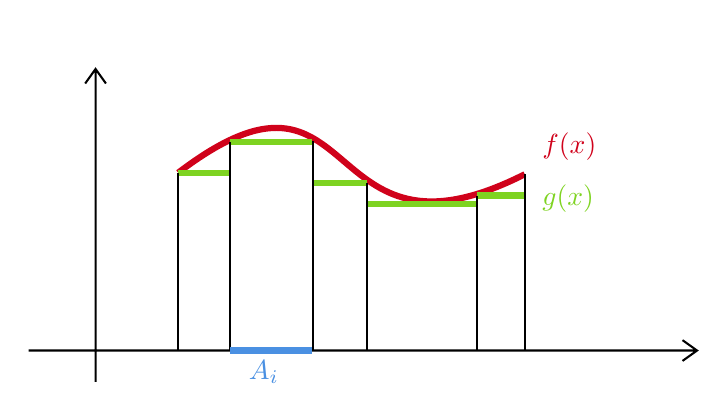
\begin{tikzpicture}[x=0.75pt,y=0.75pt,yscale=-1,xscale=1]
%uncomment if require: \path (0,171); %set diagram left start at 0, and has height of 171

%Shape: Axis 2D [id:dp6527686546165439] 
\draw  (138,140.65) -- (460,140.65)(170.2,5) -- (170.2,155.72) (453,135.65) -- (460,140.65) -- (453,145.65) (165.2,12) -- (170.2,5) -- (175.2,12)  ;
%Curve Lines [id:da4027262347286087] 
\draw [color={rgb, 255:red, 208; green, 2; blue, 27 }  ,draw opacity=1 ][line width=2.25]    (210,55) .. controls (299.8,-13.4) and (275.8,107) .. (377,55.72) ;
%Straight Lines [id:da24315154470517308] 
\draw [color={rgb, 255:red, 126; green, 211; blue, 33 }  ,draw opacity=1 ][line width=2.25]    (210,55) -- (235,55) ;
%Straight Lines [id:da22825901363329582] 
\draw [color={rgb, 255:red, 126; green, 211; blue, 33 }  ,draw opacity=1 ][line width=2.25]    (235,40) -- (274.6,40) ;
%Straight Lines [id:da5730415093182173] 
\draw [color={rgb, 255:red, 126; green, 211; blue, 33 }  ,draw opacity=1 ][line width=2.25]    (274.6,60) -- (301,60) ;
%Straight Lines [id:da5297578793317113] 
\draw [color={rgb, 255:red, 126; green, 211; blue, 33 }  ,draw opacity=1 ][line width=2.25]    (301,70) -- (327.4,70) ;
%Straight Lines [id:da9350109074443522] 
\draw [color={rgb, 255:red, 126; green, 211; blue, 33 }  ,draw opacity=1 ][line width=2.25]    (327.4,70) -- (353.8,70) ;
%Straight Lines [id:da5780729033254488] 
\draw [color={rgb, 255:red, 126; green, 211; blue, 33 }  ,draw opacity=1 ][line width=2.25]    (353.8,66) -- (377.4,66) ;
%Straight Lines [id:da7836728935339827] 
\draw    (210,140.6) -- (210,55) ;
%Straight Lines [id:da4255882760356502] 
\draw    (235,140.6) -- (235,40) ;
%Straight Lines [id:da9443315667203329] 
\draw    (275,140.6) -- (275,39.8) ;
%Straight Lines [id:da4615497493154914] 
\draw    (301,140.6) -- (301,60) ;
%Straight Lines [id:da2871328359876997] 
\draw    (354,140.6) -- (354,66) ;
%Straight Lines [id:da718006435968708] 
\draw    (377,140.6) -- (377,55.72) ;
%Straight Lines [id:da4407818981447249] 
\draw [color={rgb, 255:red, 74; green, 144; blue, 226 }  ,draw opacity=1 ][line width=2.25]    (235,140.6) -- (274.6,140.6) ;

% Text Node
\draw (384,34.4) node [anchor=north west][inner sep=0.75pt]  [color={rgb, 255:red, 208; green, 2; blue, 27 }  ,opacity=1 ]  {$f( x)$};
% Text Node
\draw (384,59.2) node [anchor=north west][inner sep=0.75pt]  [color={rgb, 255:red, 126; green, 211; blue, 33 }  ,opacity=1 ]  {$g( x)$};
% Text Node
\draw (242.6,144) node [anchor=north west][inner sep=0.75pt]  [color={rgb, 255:red, 74; green, 144; blue, 226 }  ,opacity=1 ]  {$A_{i}$};


\end{tikzpicture}
\end{figure}
\FloatBarrier

\begin{oss}
È una definizione più pulita di quella di Riemann. Il dominio e la funzione possono essere illimitati (e naturalmente l'integrale può valere $\infty $).
\end{oss}
Per definirlo per funzioni anche negative procediamo come segue.

Sia $f:A\subset \mathbb{R}^{n}\rightarrow \mathbb{C}$
\begin{equation*}
f( x) =R^{+}( x) -R^{-}( x) +I^{+}( x) -I^{-}( x)
\end{equation*}
\begin{itemize}
\item $R^{+}( x) =\max(\mathrm{Re}( f( x)) ,0) ,\forall x$
\item $R^{-}( x) =\max( -\mathrm{Re}( f( x)) ,0) ,\forall x$
\item $I^{+}( x) =\max(\mathrm{Im}( f( x)) ,0) ,\forall x$
\item $I^{-}( x) =\max( -\mathrm{Im}( f( x)) ,0) ,\forall x$
\end{itemize}

Allora definiamo
\begin{equation*}
\int _{A} f( x) dx=\int _{A} R^{+}( x) dx-\int _{A} R^{-}( x) dx+i\left[\int _{A} I^{+}( x) dx-\int _{A} I^{-}( x) dx\right]
\end{equation*}
\begin{definition}
Una funzione $f:A\subset \mathbb{R}^{n}\rightarrow \mathbb{C}$ si dice \textbf{Lebesgue-integrabile}
\begin{equation*}
\boxed{f\in L^{1} \ \ \Leftrightarrow \ \ \int _{A}| f( x)| dx< +\infty }
\end{equation*}
\end{definition}
Per esempio la funzione
\begin{equation*}
f( x) =\begin{cases}
1, & x\in \mathbb{Q}\\
0, & x\notin \mathbb{Q}
\end{cases}
\end{equation*}
non è integrabile secondo Riemann, ma il suo integrale di Lebesgue esiste e vale $0$.
\begin{oss}
Se $f( x) =g( x) ,\forall x\in A$ tranne al più un insieme di misura nulla, allora
\begin{equation*}
\int _{A} f( x) dx=\int _{A} g( x) dx\ \ \text{quasi ovunque}
\end{equation*}
\end{oss}
\begin{theorem}
[della Convergenza Monotona] Siano $f_{n} :A\rightarrow [ 0,+\infty )$. Sia $\lim\limits _{n\rightarrow +\infty } f_{n} =f( x)$ quasi ovunque, $f_{n}( x) \leqslant f_{n+1}( x) ,\forall x$ quasi ovunque e $\forall n$. Allora
\begin{equation*}
\boxed{\lim\limits _{n\rightarrow +\infty }\int _{A} f_{n}( x) dx=\int _{A}\lim\limits _{n\rightarrow +\infty } f_{n}( x) dx=\int _{A} f( x) dx}
\end{equation*}
\end{theorem}
\begin{theorem}
[della Convergenza Dominata] Siano $f_{n} :A\rightarrow \mathbb{C}$. Sia $\lim\limits _{n\rightarrow +\infty } f_{n} =f( x)$ quasi ovunque, $\exists g\in L^{1}( A)$ tale che $| f_{n}( x)| \leqslant g( x)$ quasi ovunque e $\forall n$. Allora
\begin{equation*}
\boxed{\lim\limits _{n\rightarrow +\infty }\int _{A} f_{n}( x) dx=\int _{A}\lim\limits _{n\rightarrow +\infty } f_{n}( x) dx=\int _{A} f( x) dx}
\end{equation*}
\end{theorem}
\begin{theorem}
[di Fubini] Sia $f:\mathbb{R}^{n+m}\rightarrow \mathbb{C} ,f\in L^{1}\left(\mathbb{R}^{n+m}\right)$. Sia $f=f( x,y)$ con $x\in \mathbb{R}^{n}$ e $y\in \mathbb{R}^{m}$. Allora
\begin{equation*}
\boxed{\int _{\mathbb{R}^{n+m}} f( x,y) dxdy=\int _{\mathbb{R}^{n}}\left[\int _{\mathbb{R}^{m}} f( x,y) dy\right] dx}
\end{equation*}
\end{theorem}
\section{Spazi $L^{p}$}
\begin{definition}
[Spazio $L^{p}$] Sia $A\subset \mathbb{R}^{n}$ misurabile. Sia $1\leqslant p< \infty $. Definiamo lo spazio
\begin{equation*}
L^{p}( A) =\left\{f:A\rightarrow \mathbb{C} \ \text{misurabili, tali che} \ \int _{A}| f( x)| ^{p} dx< \infty \right\}
\end{equation*}
con norma
\begin{equation*}
\Vert f\Vert _{L^{p}( A)} =\left(\int _{A}| f( x)| ^{p} dx\right)^{1/p}
\end{equation*}
\end{definition}
\begin{definition}
Se $p=\infty $ si definisce
\begin{equation*}
L^{\infty }( A) =\left\{f:A\rightarrow \mathbb{C} \ \text{misurabili, tali che} \ \exists c\geqslant 0:| f( x)| \leqslant c\ \text{q.o. in} \ A\right\}
\end{equation*}
con norma
\begin{equation*}
\Vert f\Vert _{L^{\infty }( A)} =\inf\left\{c\geqslant 0:| f( x)| \leqslant c\ \text{q.o. in} \ A\right\}
\end{equation*}
\end{definition}
\begin{definition}
[Estremo superiore essenziale] Consideriamo lo spazio $L^{\infty }( A)$, definiamo estremo superiore essenziale
\begin{equation*}
\begin{aligned}
\mathrm{ess\ sup} f( x) & =\inf\{c\in \mathbb{R} :| f( x)  >c| =0\}\\
 & =\inf\left\{c\in \mathbb{R} :| f( x)| < c\ \text{q.o. in} \ A\right\}
\end{aligned}
\end{equation*}
\end{definition}
\begin{oss}
$\Vert f\Vert _{L^{\infty }} =\mathrm{ess\ sup}| f( x)| $.
\end{oss}
\begin{theorem}
Sia $p\in [ 1,+\infty )$, $a,b\in L^{p}$, allora anche $( a+b) \in L^{p}$.
\end{theorem}
\textit{Dimostrazione.}

Sia $f( x) =| x| ^{p} ,x\geqslant 0,p >1$ è una funzione convessa, ovvero
\begin{equation*}
f( \lambda x+( 1-\lambda ) y) \leqslant \lambda f( x) +( 1-\lambda ) f( y)
\end{equation*}
poniamo $\lambda =\frac{1}{2}$ e aggiungiamo il modulo
\begin{equation*}
\left| \frac{1}{2} x+\frac{1}{2} y\right| ^{p} \leqslant \frac{1}{2}| x| ^{p} +\frac{1}{2}| y| ^{p}
\end{equation*}
integriamo
\begin{equation*}
\int \left| \frac{1}{2} x+\frac{1}{2} y\right| ^{p} dx\leqslant \frac{1}{2}\int | x| ^{p} dx+\frac{1}{2}\int | y| ^{p} dx
\end{equation*}
questo prova la tesi, se al posto di $x$ e $y$ immaginiamo che ci siano funzioni in $L^{p}$.
\begin{equation*}
\qed 
\end{equation*}
\begin{definition}
[Esponenti coniugati] Due numeri $p,q\geqslant 1$ si dicono coniugati se
\begin{equation*}
\frac{1}{p} +\frac{1}{q} =1
\end{equation*}
Poniamo inoltre
\begin{equation*}
\frac{1}{\infty } =0\ \ \ \ \frac{1}{0} =\infty 
\end{equation*}
quindi se $p=1\Rightarrow q=+\infty $, osserviamo anche che se $p\in ( 1,+\infty ) \Rightarrow q\in ( 1,+\infty )$.
\end{definition}
\begin{theorem}
[Disuguaglianza di Young] Siano $p,q$ coniugati entrambi maggiori di $1$. Allora $\forall a,b\geqslant 0$
\begin{equation*}
\frac{a^{p}}{p} +\frac{b^{q}}{q} \geqslant ab
\end{equation*}
\end{theorem}
\textit{Dimostrazione.}

La funzione logaritmo è concava, poniamo $\lambda =\frac{1}{p}$ e di conseguenza $1-\lambda =\frac{1}{q}$
\begin{gather*}
\log\left(\frac{a^{p}}{p} +\frac{b^{q}}{q}\right) \geqslant \frac{\log a^{p}}{p} +\frac{\log b^{q}}{q} =\log( ab)\\
\qed 
\end{gather*}
\begin{theorem}
[Disuguaglianza di Holder] Siano $p,q$ coniugati e siano $f\in L^{p} ,g\in L^{q}$. Allora
\begin{equation*}
f( x) g( x) \in L^{1} \ \ \text{e} \ \ \int | f( x) g( x)| dx\leqslant \Vert f\Vert _{L^{p}}\Vert g\Vert _{L^{q}}
\end{equation*}
\end{theorem}
\textit{Dimostrazione.}
\begin{itemize}
\item Se $p=1,q=+\infty $ allora $g\in L^{\infty }$ cioè $\mathrm{ess\ sup}| g( x)| < +\infty $\begin{align*}
\Rightarrow  & | g( x)| \leqslant \Vert g\Vert _{L^{\infty }} \ \ \text{q.o. in} \ x\\
\Rightarrow  & \int | f( x) g( x)| dx\leqslant \Vert g\Vert _{L^{\infty }}\int | f( x)| dx=\Vert g\Vert _{L^{\infty }}\Vert f\Vert _{L^{1}}
\end{align*}
\item Se $p,q >1$ allora\begin{equation*}
| f( x) g( x)| =\left| \lambda ^{\frac{p-1}{p}} f( x)\right| \left| \lambda ^{\frac{1-p}{p}} g( x)\right| 
\end{equation*}

Notiamo che\begin{equation*}
\frac{1}{p} +\frac{1}{q} =1\ \ \Rightarrow \ \ \frac{1}{q} =1-\frac{1}{p} =\frac{p-1}{p}
\end{equation*}

voglio utilizzare la disuguaglianza di Young\begin{align*}
\left| \lambda ^{\frac{p-1}{p}} f( x)\right| \left| \lambda ^{\frac{1-p}{p}} g( x)\right|  & \leqslant \frac{\lambda ^{\frac{p-1}{p} \cdotp p}| f( x)| ^{p}}{p} +\frac{\lambda ^{-\frac{1}{q} \cdotp q}| g( x)| ^{q}}{q}\\
 & =\frac{\lambda ^{p-1}| f( x)| ^{p}}{p} +\frac{| g( x)| ^{q}}{\lambda q}
\end{align*}

leggiamo tutta la maggiorazione\begin{equation}
\int | f( x) g( x)| dx\leqslant \frac{\lambda ^{p-1}}{p}\underbrace{\int | f( x)| ^{p} dx}_{\Vert f\Vert ^{p}_{L^{p}}} +\frac{1}{\lambda q}\underbrace{\int | g( x)| ^{q} dx}_{\Vert g\Vert ^{q}_{L^{q}}} \ \ \Rightarrow \ \ fg\in L^{1} \tag{*}
\end{equation}

Per dimostrare il risultato della disuguaglianza cerchiamo il minimo in funzione di $\lambda  >0$ derivando\begin{align*}
\frac{p-1}{p} \lambda ^{p-2}\Vert f\Vert ^{p}_{L^{p}} -\frac{1}{\lambda ^{2} q}\Vert g\Vert ^{q}_{L^{q}} & =0\\
\Rightarrow \ \ \frac{p-1}{p} \lambda ^{p}\Vert f\Vert ^{p}_{L^{p}} & =\frac{1}{q}\Vert g\Vert ^{q}_{L^{q}}\\
\lambda ^{p} & =\cancel{\frac{1}{q}}\Vert g\Vert ^{q}_{L^{q}} \cdotp \cancel{\frac{p}{p-1}} \cdotp \frac{1}{\Vert f\Vert ^{p}_{L^{p}}}\\
\lambda  & =\left[\frac{\Vert g\Vert ^{q}_{L^{q}}}{\Vert f\Vert ^{p}_{L^{p}}}\right]^{1/p}
\end{align*}

sostituendolo nella (*) otteniamo la tesi.\begin{equation*}
\qed 
\end{equation*}
\end{itemize}
\begin{theorem}
[Disuguaglianza di Minkowski] Sia $p\geqslant 1,f\in L^{p} ,g\in L^{p}$. Allora
\begin{equation*}
( f+g) \in L^{p} \ \ \text{e} \ \ \Vert f+g\Vert _{L^{p}} \leqslant \Vert f\Vert _{L^{p}} +\Vert g\Vert _{L^{p}}
\end{equation*}
\end{theorem}
\textit{Dimostrazione.}
\begin{align*}
\Vert f+g\Vert ^{p}_{L^{p}} & =\int | f( x) +g( x)| ^{p} dx\\
 & =\int | f( x) +g( x)| ^{p-1}| f( x) +g( x)| dx\\
 & \leqslant \int \underbrace{| f( x) +g( x)| ^{p-1}}_{A}\underbrace{| f( x)| }_{B} dx+\int \underbrace{| f( x) +g( x)| ^{p-1}}_{C}\underbrace{| g( x)| }_{D} dx
\end{align*}
Consideriamo $h( x) =A$
\begin{equation*}
[ h( x)]^{q} =[ h( x)]^{\frac{p}{p-1}} =| f( x) +g( x)| ^{p}
\end{equation*}
Sappiamo già, per dimostrazione precedente, che $( f+g) \in L^{p}$, allora $h\in L^{q}$. Usiamo la disuguaglianza di Holder su $A\in L^{q} ,B\in L^{p}$ e $C\in L^{q} ,D\in L^{p}$. Otteniamo
\begin{align*}
\Vert f+g\Vert ^{p}_{L^{p}} & \leqslant \Vert f\Vert _{L^{p}}\left\Vert \ | f+g| ^{p-1} \ \right\Vert _{L^{q}} +\Vert g\Vert _{L^{p}}\left\Vert \ | f+g| ^{p-1} \ \right\Vert _{L^{q}}
\end{align*}
osserviamo il termine che si presenta due volte
\begin{align*}
\left\Vert \ | f+g| ^{p-1} \ \right\Vert _{L^{q}} & =\left(\int | f( x) +g( x)| ^{( p-1) q} dx\right)^{1/q}\\
 & =\left(\int | f( x) +g( x)| ^{p} dx\right)^{1/q}\\
 & =\left(\Vert f+g\Vert ^{p}_{L^{p}}\right)^{1/q}\\
 & =\Vert f+g\Vert ^{p/q}_{L^{p}}\\
 & =\Vert f+g\Vert ^{p-1}_{L^{p}}
\end{align*}
allora
\begin{gather*}
\Vert f+g\Vert ^{p}_{L^{p}} \leqslant \Vert f\Vert _{L^{p}}\Vert f+g\Vert ^{p-1}_{L^{p}} +\Vert g\Vert _{L^{p}}\Vert f+g\Vert ^{p-1}_{L^{p}}\\
\Rightarrow \ \ \Vert f+g\Vert _{L^{p}} \leqslant \Vert f\Vert _{L^{p}} +\Vert g\Vert _{L^{p}}\\
\qed 
\end{gather*}
\begin{theorem}
Per ogni $A\subset \mathbb{R}^{n}$ misurabile, per ogni $p\in [ 1,+\infty )$, lo spazio $L^{p}( A)$ è di Banach, ed è separabile tranne nel caso $p=\infty $.
\end{theorem}
\begin{theorem}
Lo spazio $L^{2}( A)$ è uno spazio di Hilbert rispetto al prodotto scalare
\begin{equation*}
( f,g)_{2} =\int _{A} f( x)\overline{g( x)} dx
\end{equation*}
\end{theorem}
\begin{oss}
L'unico esponente coniugato con se stesso è $2$. Lo spazio $L^{2}$ è il giusto \textit{equilibrio}.
\end{oss}
\section{Serie di Fourier}

Consideriamo come spazio di lavoro $L^{2}([ -\pi ,\pi ])$.
\begin{theorem}
Consideriamo
\begin{equation*}
B=\left\{\frac{1}{\sqrt{2}} ,\cos x,\sin x,\cos( 2x) ,\sin( 2x) ,\dotsc \right\}
\end{equation*}
Consideriamo $f,g\in L^{2}([ -\pi ,\pi ])$ e definiamo il prodotto scalare
\begin{equation*}
\boxed{( f,g) =\frac{1}{\pi }\int ^{\pi }_{-\pi } f( x) g( x) dx} \ \ \text{cioè} \ \ \Vert f\Vert ^{2}_{L^{2}} =\frac{1}{\pi }\int ^{\pi }_{-\pi } f^{2}( x) dx
\end{equation*}
allora $B$ è una base di Hilbert.
\end{theorem}
Si vede facilmente che i suoi vettori sono normali
\begin{gather*}
\left\Vert \frac{1}{\sqrt{2}}\right\Vert =\frac{1}{\pi }\int ^{\pi }_{-\pi }\left(\frac{1}{\sqrt{2}}\right)^{2} dx=1\\
\Vert \sin( kx)\Vert =\frac{1}{\pi }\int ^{\pi }_{-\pi }(\sin( kx))^{2} dx=1
\end{gather*}
e ortogonali a due a due
\begin{equation*}
\frac{1}{\pi }\int ^{\pi }_{-\pi }\frac{1}{\sqrt{2}}\sin( kx) dx=0\ \ \ \ \frac{1}{\pi }\int ^{\pi }_{-\pi }\cos( kx)\cos( jx) dx=0,\ \forall j\neq k
\end{equation*}
Vale inoltre, dalla teoria degli spazi di Hilbert, la seguente relazione, che ci permette di costruire ogni elemento dello spazio di Hilbert tramite la base
\begin{equation*}
\forall f\in L^{2}([ -\pi ,\pi ]) ,\ \ f( x)\textcolor[rgb]{0.82,0.01,0.11}{=}\frac{a_{0}}{\sqrt{2}} +\sum\limits ^{\infty }_{n=1}[ a_{n}\cos( nx) +b_{n}\sin( nx)]
\end{equation*}
Cerchiamo l'espressione per calcolare i coefficienti, e soprattutto cerchiamo di capire in che senso vale tale uguaglianza in rosso.

Sappiamo che i coefficienti si calcolano come prodotto scalare della cosa da costruire (la funzione in $L^{2}$ nel nostro caso) per il rispettivo elemento della base
\begin{gather*}
a_{n} =( f,e_{n}) =\frac{1}{\pi }\int ^{\pi }_{-\pi } f( x)\cos( nx) dx\\
b_{n} =( f,e_{n}) =\frac{1}{\pi }\int ^{\pi }_{-\pi } f( x)\sin( nx) dx\\
a_{0} =\frac{1}{\pi }\int ^{\pi }_{-\pi } f( x) \cdotp \textcolor[rgb]{0.29,0.56,0.89}{\frac{1}{\sqrt{2}}} dx
\end{gather*}
Possiamo "togliere" dalla formula il termine blu e accorparlo nella formula completa, in modo da non avere radici, otteniamo la formula per le serie di Fourier\footnote{L'importanza della serie di Fourier è cruciale nelle equazioni differenziali. Infatti, nell'equazione del calore, che deriva direttamente dal postulato di Fourier, la soluzione si trova facilmente se è composta da soli seni. In questo modo si può costruire facilmente la soluzione usando una serie di Fourier, che sarà ancora soluzione per il principio di sovrapposizione delle equazioni differenziali. Fourier, quando sviluppò questa teoria, stava proprio cercando di risolvere questo problema, e grazie ciò, ottenne la sua \textit{immortalità}.}
\begin{equation*}
\boxed{\forall f\in L^{2}([ -\pi ,\pi ]) ,\ \ f( x) =\frac{a_{0}}{2} +\sum\limits ^{\infty }_{n=1}[ a_{n}\cos( nx) +b_{n}\sin( nx)]}
\end{equation*}
\begin{oss}
[Convergenza $L^{2}$] L'uguaglianza vale in senso $L^{2}$, ovvero che se indichiamo con $S_{N}( x)$ le somme parziali
\begin{equation*}
S_{N}( x) =\frac{a_{0}}{2} +\sum\limits ^{N}_{n=1}[ a_{n}\cos( nx) +b_{n}\sin( nx)]
\end{equation*}
vale il limite\footnote{come di consueto, dire che qualcosa si avvicina a un'altra cosa, è equivalente a dire che \textit{una certa norma} della differenza tra le due tende a zero.}
\begin{equation*}
\lim\limits _{N\rightarrow +\infty }\int ^{\pi }_{-\pi }[ f( x) -S_{N}( x)]^{2} dx=0
\end{equation*}
\end{oss}
\begin{oss}
La funzione che scegliamo di approssimare deve essere periodica di periodo $2\pi $, si può chiaramente generalizzare il risultato a periodi generici $T$
\begin{equation*}
\forall f\in L^{2}\left(\left[ -\frac{T}{2} ,\frac{T}{2}\right]\right) ,\ \ f( x) =\frac{a_{0}}{2} +\sum\limits ^{\infty }_{n=1}\left[ a_{n}\cos\left(\frac{2n\pi }{T} x\right) +b_{n}\sin\left(\frac{2n\pi }{T} x\right)\right]
\end{equation*}
con prodotto scalare
\begin{equation*}
( f,g) =\frac{1}{\frac{T}{2}}\int ^{T/2}_{-T/2} f( x) g( x) dx
\end{equation*}
quindi per esempio
\begin{equation*}
a_{n} =\frac{2}{T}\int ^{T/2}_{-T/2} f( x)\cos\left(\frac{2n\pi }{T} x\right) dx
\end{equation*}
\end{oss}
\begin{oss}
[Convergenza uniforme] Dal momento che
\begin{equation*}
| a_{n}\cos( nx) +b_{n}\sin( nx)| \leqslant | a_{n}| +| b_{n}| 
\end{equation*}
Per il test di Weierstrass vale la seguente relazione che ci permette di stabilire se la serie converge uniformemente
\begin{equation*}
\sum\limits ^{\infty }_{n=1}(| a_{n}| +| b_{n}| ) < \infty \ \ \Rightarrow \ \ f( x) \ \text{converge uniformemente}
\end{equation*}
\end{oss}
\textit{Esempio.}

Sia $f( x) =| x| $ nell'intervallo $[ -\pi ,\pi ]$ estesa con periodicità a tutto $\mathbb{R}$, calcoliamo lo sviluppo di Fourier.
\begin{align*}
a_{n} & =\frac{1}{\pi }\int ^{\pi }_{-\pi }| x| \cos( nx) dx=\frac{2}{\pi }\int ^{\pi }_{0} x\cos( nx) dx\\
 & =\frac{2}{\pi }\left\{\cancel{x\cdotp \left. \frac{\sin( nx)}{n}\right| ^{\pi }_{0}} -\int ^{\pi }_{0}\frac{\sin( nx)}{n} dx\right\}\\
 & =\frac{2}{\pi }\left\{\left. \frac{\cos( nx)}{n^{2}}\right| ^{\pi }_{0}\right\} =\frac{2}{\pi n^{2}}\left[( -1)^{n} -1\right]\\
 & \\
b_{n} & =\frac{1}{\pi }\int ^{\pi }_{-\pi }| x| \sin( nx) dx=0\\
 & \\
a_{0} & =\frac{2}{\pi }\int ^{\pi }_{0} xdx=\pi 
\end{align*}
allora si scrive in serie di Fourier
\begin{equation*}
| x| =\frac{\pi }{2} +\sum\limits ^{\infty }_{n=1}\frac{2}{\pi n^{2}}\left[( -1)^{n} -1\right]\cos( nx)
\end{equation*}
\begin{definition}
Una funzione $f:[ -\pi ,\pi ]\rightarrow \mathbb{R}$ si dice \textbf{regolare a tratti} se è derivabile e ha un numero finito di punti di discontinuità $\{x_{n}\}_{n=1\dotsc N}$ e in tali punti esistono finiti i limiti
\begin{equation*}
\lim\limits _{x\rightarrow x^{+}_{n}} f( x) \ \ \ \ \ \ \lim\limits _{x\rightarrow x^{-}_{n}} f( x)
\end{equation*}
Escludiamo quindi asintoti, punti di cuspide, ma i limiti possono eventualmente essere diversi.
\end{definition}
\begin{theorem}
[Convergenza puntuale] Una funzione $f:[ -\pi ,\pi ]\rightarrow \mathbb{R}$ regolare a tratti. Allora la serie di Fourier converge $\forall x\in [ -\pi ,\pi ]$ tale che $f( x)$ è continua. Nei punti in cui non è continua invece converge al valore medio tra i due limiti.
\end{theorem}
\begin{theorem}
[Derivazione] Per la derivazione possiamo dire che
\begin{equation*}
f'( x) =\sum\limits ^{\infty }_{n=1}[ -na_{n}\sin( nx) +nb_{n}\cos( nx)]
\end{equation*}
osserviamo che
\begin{equation*}
\sup _{x\in [ -\pi ,\pi ]}[ -na_{n}\sin( nx) +nb_{n}\cos( nx)] \leqslant n(| a_{n}| +| b_{n}| )
\end{equation*}
per cui per il test di Weierstrass se
\begin{equation*}
\sum\limits ^{\infty }_{n=1} n(| a_{n}| +| b_{n}| ) < \infty \ \ \Rightarrow \ \ f'( x) \ \text{converge uniformemente}
\end{equation*}
e naturalmente anche $f( x)$. La condizione \textit{sufficiente} affinché la serie di Fourier sia derivabile $k$ volte è che
\begin{equation*}
\sum\limits ^{\infty }_{n=1} n^{k}(| a_{n}| +| b_{n}| ) < \infty 
\end{equation*}
\end{theorem}
\begin{oss}
Lo usiamo normalmente solo come controllo per sapere se abbiamo calcolato bene la serie di Fourier, di solito sappiamo già se $f$ è derivabile o meno.
\end{oss}
Esiste una base alternativa, che troviamo se scriviamo le relazioni complesse
\begin{equation*}
\cos( nx) =\frac{e^{inx} +e^{-inx}}{2} \ \ \ \ \ \ \ \ \sin( nx) =\frac{e^{inx} -e^{-inx}}{2i}
\end{equation*}
allora la serie di Fourier si scrive nella sua \textbf{forma esponenziale}
\begin{equation*}
f( x) =\frac{a_{0}}{2} +\sum\limits ^{\infty }_{n=1}\left[ a_{n}\frac{e^{inx} +e^{-inx}}{2} +b_{n}\frac{e^{inx} -e^{-inx}}{2i}\right] \ \ \Rightarrow \ \ \boxed{f( x) =\sum\limits ^{\infty }_{n=-\infty } c_{n} e^{inx}}
\end{equation*}
\begin{oss}
In generale questi coefficienti sono complessi $c_{n} =\overline{c_{-n}}$.
\end{oss}
\begin{oss}
La base $\left\{e^{inx}\right\}_{n\in \mathbb{Z}}$ è una base ortonormale
\begin{equation*}
\int ^{\pi }_{-\pi } e^{inx} e^{imx} dx=\int ^{\pi }_{-\pi } e^{i( n-m) x} dx=\begin{cases}
2\pi , & n=m\\
\left. \frac{e^{i( n-m) x}}{i( n-m)}\right| ^{\pi }_{-\pi } =0, & n\neq m
\end{cases}
\end{equation*}
normalizziamo, quindi il prodotto scalare sarà
\begin{equation*}
( f,g) =\frac{1}{2\pi }\int ^{\pi }_{-\pi } f( x)\overline{g( x)} dx
\end{equation*}
e i coefficienti saranno
\begin{equation*}
c_{n} =\frac{1}{2\pi }\int ^{\pi }_{-\pi } f( x) e^{-inx} dx
\end{equation*}
Il $-$ è dovuto al fatto che $g$ è coniugato nel prodotto scalare.
\end{oss}




\chapter{Distribuzioni}

\section{Spazi di Banach e spazi duali}

Per arrivare a definirle e vedere a cosa servono dobbiamo fare alcuni passaggi preliminari. Definiamo il concetto di spazio duale. Parliamo di spazio duale non necessariamente, ma specialmente nel contesto degli spazi di Banach.

Supponiamo di avere due spazi di Banach $X,Y$ in modo assolutamente generale, poi ci concentreremo su uno specifico.
\begin{definition}
[Linearità] Possiamo considerare tutte le funzioni lineari da $X$ in $Y$
\begin{equation*}
L:X\rightarrow Y\ \ \ \ L( \alpha x_{1} +\beta x_{2}) =\alpha L( x_{1}) +\beta L( x_{2})
\end{equation*}
\end{definition}
Teniamo presente che quando parliamo di spazi di Banach spesso intendiamo spazi a dimensione infinita, in questo caso certe idee che abbiamo molto naturali e intuitive delle funzioni lineari non valgono necessariemente. In particolare la continuità \textbf{non} è necessariamente garantita in caso di funzioni lineari. In uno spazio di Banach possiamo avere funzioni lineari continue e funzioni lineari non continue. 
\begin{definition}
[Continuità] Una funzione è continua se
\begin{equation*}
x_{n}\rightarrow x\ \ \Rightarrow \ \ L( x_{n})\rightarrow L( x)
\end{equation*}
\end{definition}
Ricordiamo un'altra definizione non scontata negli spazi a dimensione infinita
\begin{definition}
[Limitatezza] Una funzione lineare è limitata se
\begin{equation*}
\exists c\ \ \Vert L( x)\Vert \leqslant c\Vert x\Vert \ \ \forall x\in X
\end{equation*}
\end{definition}
Vale un teorema che collega queste due definizioni.
\begin{theorem}
Siano $X,Y$ due spazi di Banach qualsiasi. Una funzione lineare $L:X\rightarrow Y$ è limitata se e solo se è continua.
\end{theorem}
Quello che ci interessa è un tipo particolare di funzioni tra spazi di Banach. Il secondo spazio sarà $\mathbb{R}$, che è esso stesso uno spazio di Banach, è uno spazio lineare dotato di norma (il valore assoluto) e continuo rispetto a questa norma.
\begin{equation*}
L:X\rightarrow \mathbb{R} \ \ \ \ X\ \text{di Banach}
\end{equation*}
\begin{definition}
Dato uno spazio $X$ di Banach, si dice \textbf{spazio duale} l'insieme di tutte le \underline{funzioni lineari continue} da $X$ in $\mathbb{R}$. Queste funzioni si chiamano anche \textbf{funzionali}. 
\end{definition}
Supponiamo per esempio che $X$ sia $\mathbb{R}^{n}$, possiamo considerare tutte le funzioni lineari (e quindi continue, essendo $\mathbb{R}^{n}$ a dimensione finita)
\begin{equation*}
L:\mathbb{R}^{n}\rightarrow \mathbb{R}
\end{equation*}
Come possiamo descriverle tutte? Le identifichiamo con il prodotto scalare con un altro vettore. Dato $y\in \mathbb{R}^{n}$ possiamo definire $L( x) :=( y,x)$. Per esempio il duale di $\mathbb{R}^{n}$ è $\mathbb{R}^{n}$ stesso.

La categoria più importante di spazi di Banach che abbiamo visto fin'ora è $L^{p}$, cos'è il suo duale? Abbiamo un modo molto semplice.
\begin{theorem}
Se $1< p< +\infty $, allora il duale di $L^{p}$ è $L^{q}$ dove $q$ è l'esponente coniugato di $p$: $\frac{1}{p} +\frac{1}{q} =1$.
\end{theorem}
Sia $f\in L^{p}$ e $L( f) \in \mathbb{R}$, possiamo dimostrare che $\forall L$ funzionale lineare su $L^{p}$ esiste una funzione $h\in L^{q}$ tale che $L( f) =\int hf$. Non stiamo specificando in quale dominio stiamo definendo questi spazi. Grazie alla disuguaglianza di Holder otteniamo questo risultato. Non indaghiamo ulteriormente.

Torniamo alla definizione di duale. Una possibile notazione dello spazio duale di $X$ è $X'$. Questo spazio duale è lui stesso uno spazio di Banach. È ovviamente uno spazio vettoriale, ma dobbiamo far vedere che c'è una \textit{norma}. Un elemento del duale è un funzionale $L:X\rightarrow \mathbb{R}$, questo vuol dire che dato un elemento $x\in X$ allora $L( x) \in \mathbb{R}$
\begin{equation*}
\Vert L\Vert =\sup _{\Vert x\Vert =1}| L( x)| 
\end{equation*}
È vero che questo è effettivamente un numero reale? Abbiamo detto che il duale è fatto da funzionali lineari continui, ovvero limitati, quindi sicuramente questo estremo superiore è limitato. La definizione di poco fa di funzione limitata era che $\exists c$ tale che $| L( x)| \leqslant c\Vert x\Vert $, quindi sicuramente questo estremo superiore è minore di $c$. Si tratta di far vedere che è effettivamente una norma, abbiamo allora questo teorema.
\begin{theorem}
Sia $X$ spazio di Banach. Allora $X'$ è uno spazio di Banach lui stesso rispetto alla norma
\begin{equation*}
\Vert L\Vert =\sup _{\Vert x\Vert =1}| L( x)| 
\end{equation*}
\end{theorem}
\begin{definition}
[Supporto di una funzione] Supponiamo ora di avere una funzione $f:A\subset \mathbb{R}^{n}\rightarrow \mathbb{R}$. Si dice supporto di $f$ l'insieme
\begin{equation*}
\mathrm{supp} f=\overline{\{x\in A,f( x) \neq 0\}}
\end{equation*}
È la chiusura dell'insieme dei punti dove la funzione non si annulla.
\end{definition}
Diamo la definizione di un nuovo spazio vettoriale, se abbiamo $A\subset \mathbb{R}^{n}$ sappiamo cos'è $L^{p}( A)$.
\begin{definition}
Si dice $L^{p}_{\mathrm{loc}}$ l'insieme delle funzioni $f:A\rightarrow \mathbb{R}$ tali che $\forall K\subset A$ compatto
\begin{equation*}
\exists \ \ \int _{K}| f| ^{p} dx\ \ \text{finito} .
\end{equation*}
\end{definition}
È molto più grande dello spazio $L^{p}$.

\section{Funzioni test e distribuzioni}
Adesso dobbiamo definire un nuovo spazio di funzioni, che non è uno spazio di Banach.
\begin{definition}
[Spazio delle funzioni test] Sia $A\subset \mathbb{R}^{n}$ aperto. Chiamiamo funzioni $C^{\infty }$ a supporto compatto, o funzioni test, e lo indichiamo con $\mathcal{D}( A)$ l'insieme delle funzioni $f:A\rightarrow \mathbb{R}$, derivabili infinite volte $f\in C^{\infty }$ e tali che il supporto $\mathrm{supp} f$ è compatto.
\end{definition}
Una funzione in $\mathcal{D}( A)$ viene detta \textbf{funzione test}. Queste funzioni sono un insieme estremamente piccolo. Non è banale neanche fare degli esempi in $\mathcal{D}(\mathbb{R})$. Per esempio
\begin{equation*}
f( x) =\begin{cases}
e^{\frac{1}{x^{2} -1}} & | x| < 1\\
0 & | x| \geqslant 1
\end{cases}
\end{equation*}
Somiglia a una gaussiana, ma fuori da $[ -1,1]$ si annulla.

\fg{0.7}{esempioFunzioneD}

Non è banale che sia $C^{\infty }$ nei punti $-1,1$, ma si può dimostrare.

Nessuna funzione elementare appartiene a questo insieme.

Questo insieme non è uno spazio di Banach, se definiamo una norma, non può essere uno spazio di Banach rispetto a quella norma. Nonostante ciò vogliamo definire un concetto di convergenza.

Daremo le prossime definizioni in dimensione $1$ per alleggerire le notazioni.
\begin{definition}
[Convergenza in $\mathcal{D}$]Sia $A\subset \mathbb{R}$ aperto e consideriamo l'insieme $\mathcal{D}( A)$, consideriamo una successione di funzioni $\{f_{n}\} \subset \mathcal{D}( A)$. Diciamo che $f_{n}\rightarrow f$ in $\mathcal{D}( A)$ se
\begin{enumerate}
	\item $\exists K\subset A$ compatto tale che il supporto $\mathrm{supp} f_{n} \subset K$, ciascuna funzione è a supporto compatto, ma vogliamo che esista un compatto che contenga i supporti di tutte le funzioni.
	\item $\forall k\in \mathbb{N}$ la derivata di ordine $k$ della successione di funzioni converge alla derivata di ordine $k$ della funzione uniformemente $f^{( k)}_{n}\rightarrow f^{( k)}$.
\end{enumerate}
\end{definition}
Si può dimostrare che non possiamo definire questa convergenza in norma o distanza, motivo per cui l'abbiamo definita noi così. Ora possiamo finalmente arrivare alla definizione di distribuzione.
\begin{definition}
[Distribuzione] Sia $A\subset \mathbb{R}$ aperto. Chiamiamo \textbf{distribuzione} in $A$ un funzionale (lineare e continuo) su $\mathcal{D}( A)$. Quindi lo spazio delle distribuzione è il suo duale $\mathcal{D} '( A)$.
\end{definition}
Stiamo cercando di generalizzare il concetto di funzione.
\begin{theorem}
A ogni funzione $u\in L^{1}_{\mathrm{loc}}( A)$ corrisponde una distribuzione in $\mathcal{D} '( A)$.

Indichiamo con $( u,f)$ il prodotto di dualità, cioè la distribuzione (funzionale lineare e continuo) associata ad $u$ che agisce sulla funzione test $f$
\begin{equation*}
\boxed{( u,f) =\int _{A} ufdx} \ \ \ \ u\in L^{1}_{\mathrm{loc}}( A) \ \ f\in \mathcal{D}( A)
\end{equation*}
\end{theorem}
\textit{Dimostrazione.}

Dobbiamo verificare che l'integrale sia ben definito, lineare e continuo (o limitato).
\begin{itemize}
\item \textit{ben definito.} Il supporto di $f$ è un certo insieme $K\subset A$ compatto, quindi si annulla al di fuori di $K$, allora\begin{equation*}
\int _{A} ufdx=\int _{K} ufdx
\end{equation*}ma $f$ è anche limitata (essendo continua a supporto compatto) e $u\in L^{1}_{\mathrm{loc}}$:\begin{equation*}
\left| \int _{K} ufdx\right| \leqslant \sup | f| \left| \int _{K} udx\right| < +\infty 
\end{equation*}
\item \textit{lineare}, infatti\begin{equation*}
( u,c_{1} f_{1} +c_{2} f_{2}) =\int _{A} u( c_{1} f_{1} +c_{2} f_{2}) dx
\end{equation*}per la linearità dell'integrale\begin{equation*}
\int _{A} u( c_{1} f_{1} +c_{2} f_{2}) dx=c_{1}\int _{A} uf_{1} dx+c_{2}\int _{A} uf_{2} dx=c_{1}( u,f_{1}) +c_{2}( u,f_{2})
\end{equation*}
\item \textit{continuo, o limitato} (sono equivalenti). Per ipotesi $f_{n}\rightarrow f$ in $\mathcal{D}( A)$ e $u\in L^{1}_{\mathrm{loc}}$. Allora la convergenza in $\mathcal{D}( A)$ garantisce che il supporto di tutte le $f_{n}$ sia contenuto in un compatto $K\subset A$, e inoltre $f_{n}\rightarrow f$ (e le derivate) uniformemente, cioè $\Vert f_{n} -f\Vert _{\infty }\rightarrow 0$. Per definizione di $L^{1}_{\mathrm{loc}}$ la funzione $u$ ristretta al compatto $K$ è $L^{1}( K)$. Possiamo allora usare la disuguaglianza di Holder con $p=1,q=\infty $ per far vedere che\begin{equation*}
\left| \int _{K} u( f_{n} -f) dx\right| \leqslant \Vert u\Vert _{L^{1}( K)}\Vert f_{n} -f\Vert _{\infty }\rightarrow 0
\end{equation*}allora abbiamo fatto vedere che\begin{equation*}
\int _{A} u( f_{n} -f) dx\rightarrow 0\ \ \ \ \Leftrightarrow \ \ \ \ \int _{A} uf_{n} dx\rightarrow \int _{A} ufdx
\end{equation*}quindi qualsiasi funzione $L^{1}_{\mathrm{loc}}$ è una distribuzione su quell'insieme.\begin{equation*}
\qed 
\end{equation*}
\end{itemize}

Si noti che lo spazio $L^{1}_{\mathrm{loc}}$ è molto più grande di $L^{1}$, ad esempio banalmente qualunque polinomio non identicamente nullo non è integrabile su tutto $\mathbb{R}$, ma è integrabile su qualunque compatto.

Tutte le distribuzioni si possono vedere come associate a una funzione $L^{1}_{\mathrm{loc}}$? No, vediamo un controesempio con la \textbf{delta di Dirac}, che definiamo come distribuzione su $\mathbb{R}$. Ad ogni funzione $f\in \mathcal{D}(\mathbb{R})$ e $y\in \mathbb{R}$ vogliamo associare una distribuzione $\delta _{y} \in \mathcal{D} '(\mathbb{R})$
\begin{equation*}
\boxed{( \delta _{y} ,f) =f( y) \in \mathbb{R}}
\end{equation*}
\textit{Dimostrazione.}
\begin{itemize}
\item ha valori in $\mathbb{R}$, $\delta _{y} :\mathcal{D}(\mathbb{R})\rightarrow \mathbb{R}$
\item è lineare $( \delta _{y} ,c_{1} f_{1} +c_{2} f_{2}) =( c_{1} f_{1} +c_{2} f_{2})( y) =c_{1} f_{1}( y) +c_{2} f_{2}( y)$ che è proprio uguale a $c_{1}( \delta _{y} ,f_{1}) +c_{2}( \delta _{y} ,f_{2})$
\item è continua. Sia $f_{n}\rightarrow f$, cioè il supporto di tutte le $f_{n}$ è contenuto in $K$ compatto e $f_{n}\rightarrow f$ uniformemente, e quindi anche puntualmente:
\begin{itemize}
\item se $y\notin K$ allora $( \delta _{y} ,f_{n}) =0$ e $( \delta _{y} ,f) =0$
\item se $y\in K$ allora $( \delta _{y} ,f_{n}) =f_{n}( y)\rightarrow f( y) =( \delta _{y} ,f)$
\end{itemize}

\begin{equation*}
\qed 
\end{equation*}
\end{itemize}
Spesso si scrive
\begin{equation*}
( \delta _{y} ,f) =\int _{\mathbb{R}} \delta _{y}( x) f( x) dx=f( y)
\end{equation*}
La delta di Dirac nasce per estrarre in modo semplice il valore di una funzione in un punto, e da qui si è poi sviluppata la teoria delle distribuzioni. Ad ogni funzione $L^{1}_{\mathrm{loc}}$ si può quindi associare una distribuzione, ma non viceversa, le distribuzioni sono di più.

Un altro modo di interpretare la delta di Dirac è il limite di una gaussiana
\begin{equation*}
f( x) =\frac{1}{\sqrt{2\pi }} e^{-\frac{1}{2} x^{2}} \ \ \ \ \Vert f\Vert _{L^{1}} =1
\end{equation*}
definiamo
\begin{equation*}
f_{n}( x) =nf( nx)
\end{equation*}
\fg{0.7}{deltaGaussianaLimite}

dove
\begin{equation*}
\Vert f_{n}\Vert _{L^{1}} =\int _{\mathbb{R}}| f_{n}( x)| dx=\int _{\mathbb{R}} nf( nx) dx
\end{equation*}
chiamo $y=nx$ allora $dy=ndx$
\begin{equation*}
\int _{\mathbb{R}} nf( nx) dx=\int _{\mathbb{R}} f( y) dy=1
\end{equation*}
Notiamo che
\begin{equation*}
f_{n}( x) =\frac{n}{\sqrt{2\pi }} e^{-\frac{1}{2}( nx)^{2}}\xrightarrow{n\rightarrow \infty } 0\ \ \forall x\neq 0
\end{equation*}
Essendo $L^{1}$, quindi anche $L^{1}_{\mathrm{loc}}$, le possiamo vedere come distribuzioni. Possiamo dimostrare che $\forall \varphi \in \mathcal{D}( A)$, $( f_{n} ,\varphi )\rightarrow ( \delta _{0} ,\varphi )$.



Più uno spazio è piccolo e più il suo duale è grande, e viceversa. Lo spazio $\mathcal{D}( A)$ è molto piccolo, quindi il duale (lo spazio delle distribuzioni) sarà molto grande, ma pur essendo molto grande, avrà delle proprietà molto forti (derivabilità infinita). \textit{Stiamo cercando capre e cavoli}.


\begin{definition}
[Convergenza di una distribuzione] Cosa vuol dire avere una successione di distribuzioni $\{\Lambda _{n}\}$ che converge a $\Lambda $ \underline{nel senso delle distribuzioni}? Come prima, se $\forall \varphi \in \mathcal{D}( A) \Rightarrow ( \Lambda _{n} ,\varphi )\rightarrow ( \Lambda ,\varphi )$. La definizione è simmetrica rispetto all'altra.
\end{definition}
Veniamo al supporto. Una distribuzione non ha una variabile, non si annulla come una funzione, non è una funzione.
\begin{definition}
[Supporto di una distribuzione] Sia $\Lambda \subset \mathcal{D} '( A)$. Consideriamo $B\subset A$ e $\varphi \in \mathcal{D}( B)$. Supponiamo che $( \Lambda ,\varphi ) =0\ \ \forall \varphi $. Questo è il modo per dire che "si annulla", diciamo
\begin{equation*}
\boxed{
	\mathrm{supp} \Lambda =
	\left(\bigcup_{\substack{B\subset A\\B\text{ aperti}} } \{B:(\Lambda,\varphi)=0,\ \forall \varphi \in \mathcal{D}(B)\}\right)^{C}
}
\end{equation*}
\end{definition}


NB. Quando diciamo che a $u\in L^{1}_{\mathrm{loc}}( A)$ corrisponde una distribuzione, diciame che esiste una $\Lambda _{u}$ distribuzione definita come $( \Lambda _{u} ,\varphi ) =\int _{A} u\varphi $, ma talvolta scriveremo direttamente $u$ con abuso di notazione.
\begin{definition}
[Derivata di una distribuzione] Sia $\Lambda \in \mathcal{D} '( A)$ una distribuzione. Definiamo la sua distribuzione derivata $\Lambda '\in \mathcal{D} '( A)$. Per ogni $\varphi \in \mathcal{D}( A)$ dobbiamo definire quanto vale $( \Lambda ',\varphi )$
\begin{equation*}
\boxed{( \Lambda ',\varphi ) =-( \Lambda ,\varphi ')}
\end{equation*}
\end{definition}
Questo somiglia molto all'integrazione per parti (in realtà è molto più che una somiglianza). Controlliamo che sia una distribuzione
\begin{itemize}
\item definita $\Lambda ':\mathcal{D}( A)\rightarrow \mathbb{R}$, sì per come è costruita, $\varphi '$ è comunque definito essendo $C^{\infty }$ a supporto compatto
\item lineare:\begin{equation*}
( \Lambda ',a_{1} \varphi _{1} +a_{2} \varphi _{2}) =a_{1}( \Lambda ',\varphi _{1}) +a_{2}( \Lambda ',\varphi _{2})
\end{equation*}
\item continuo:\begin{equation*}
\varphi _{k}\rightarrow \varphi \ \ \text{in} \ \mathcal{D}( A) \ \ \Rightarrow \ \ ( \Lambda ',\varphi _{k})\rightarrow ( \Lambda ',\varphi )
\end{equation*}

infatti, dato che $\varphi '_{k}\rightarrow \varphi '$\begin{gather*}
( \Lambda ',\varphi _{k}) =-( \Lambda ,\varphi '_{k})\rightarrow -( \Lambda ,\varphi ') =( \Lambda ',\varphi )\\
\qed 
\end{gather*}
\end{itemize}

Andiamo ora a capire che ha le stesse proprietà di una derivata. Consideriamo una funzione derivabile $u\in C^{1}( A) \subset L^{1}_{\mathrm{loc}}( A)$, ma allora è associata ad una distribuzione, che continueremo a chiamare $u$
\begin{equation*}
( u,\varphi ) =\int _{A} u( x) \varphi ( x) dx
\end{equation*}
Sappiamo che esiste $u'\in C^{0}( A) \subset L^{1}_{\mathrm{loc}}$, associata a sua a volta ad una distribuzione
\begin{gather*}
\underbrace{( u',\varphi ) =-( u,\varphi ')}_{\text{definizione di prima}}\\
( u',\varphi ) =\int _{A} u'( x) \varphi ( x) dx=\cancel{u( b) \varphi ( b)} -\cancel{u( a) \varphi ( a)} -\int ^{b}_{a} u( x) \varphi '( x) dx\ \ \ \ A=[ a,b]
\end{gather*}
i termini si cancellano perché $\varphi $ è a supporto compatto, che è contenuto in $A$, quindi $\varphi $ si annulla agli estremi $\varphi ( a) =0=\varphi ( b)$.



\textit{Esempio.}

Consideriamo la funzione
\fg{0.6}{rampa}
\begin{equation*}
u( x) =\begin{cases}
x & x\geqslant 0\\
0 & x< 0
\end{cases}
\end{equation*}
Non è derivabile nell'origine, ma è $L^{1}_{\mathrm{loc}}$, quindi derivabile nel senso delle distribuzioni. Sia $\varphi \in \mathcal{D}(\mathbb{R})$
\begin{equation*}
( u',\varphi ) =-( u,\varphi ') =-\int _{\mathbb{R}} u( x) \varphi '( x) dx=-\int ^{M}_{0} x\varphi '( x) dx
\end{equation*}
$M$ perché $\varphi $ è a supporto compatto, quindi ci sarà un $M$; applico l'integrazione per parti
\begin{align*}
-\int ^{M}_{0} x\varphi '( x) dx & =-\cancel{[ x\varphi ( x)]^{M}_{0}} +\int ^{M}_{0} \varphi ( x) dx=\int ^{M}_{0} \varphi ( x) dx\\
 & =\int ^{+\infty }_{0} \varphi ( x) dx=\int _{\mathbb{R}} H( x) \varphi ( x) dx=( H,\varphi )
\end{align*}
dove $H( x)$ è la \textbf{funzione di Heaviside}, che abbiamo interpretato come distribuzione
\begin{equation*}
H( x) =\begin{cases}
1 & x\geqslant 0\\
0 & x< 0
\end{cases}
\end{equation*}
NB. Tutto quello che vediamo riguardante gli spazi $L^{p}$ riguarda gli integrali, quindi che valga $0$ o $1$ quando $x=0$ è del tutto irrilevante.

Allora la derivata di $u$, cioè $u'$, nel senso delle distribuzioni, è $H$.

Sembra che non abbiamo fatto granché se non togliere di mezzo un punto angoloso: spingiamoci oltre e deriviamo la funzione di Heaviside, che non è nemmeno continua.
\begin{align*}
( H',\varphi ) & =-( H,\varphi ') \ \ \forall \varphi \in \mathcal{D}(\mathbb{R})\\
 & =-\int _{\mathbb{R}} H( x) \varphi '( x) dx=-\int ^{+\infty }_{0} \varphi '( x) dx\\
 & =\varphi ( 0) -\lim _{x\rightarrow +\infty } \varphi ( x) =\varphi ( 0) =( \delta _{0} ,\varphi )
\end{align*}
La derivata di $H$ nel senso delle distribuzioni è la distribuzione delta di Dirac (centrata nel punto di discontinuità). Può sembrare strano derivare la delta, ma si può fare.
\begin{equation*}
( \delta '_{a} ,\varphi ) =-( \delta _{a} ,\varphi ') =-\varphi '( a)
\end{equation*}
estendiamo a un ordine $n$
\begin{equation*}
\left( \delta ^{( n)}_{a} ,\varphi \right) =( -1)^{n} \varphi ^{( n)}( a)
\end{equation*}
\section{Funzioni a decrescita rapida e distribuzioni temperate}

Lo spazio delle $\varphi $ è lo spazio delle funzioni test, delle funzioni $C^{\infty }$ a supporto compatto, uno spazio molto stringente. Cerchiamo di allentarlo un po' introducendo un nuovo spazio chiamato \textbf{spazio delle funzioni a decrescita rapida} (o \textbf{spazio di Schwartz}\footnote{Si noti che si tratta di un matematico differente da quello del teorema sulle derivate seconde, Karl Hermann Amandus Schwarz (1843-1921). Qui si parla di Laurent Schwartz (1915-2002), medaglia Fields nel 1950.}).
\begin{definition}
[Spazio delle funzioni a decrescita rapida] Diciamo che $f\in \mathcal{S}(\mathbb{R})$ se $\boxed{f\in C^{\infty }}$ e $\boxed{x^{k} f^{( n)}( x)}$ è \underline{limitata} $\forall k,n\in \mathbb{N}$.
\end{definition}
Le definiamo su tutto $\mathbb{R}$. Non chiediamo che si annullino fuori da un compatto, ma che si annullino più rapidamente di qualsiasi polinomio insieme a tutte le derivate per $x\rightarrow \pm \infty $. Una gaussiana per esempio tende a $0$ più velocemente di qualsiasi polinomio con le sue derivate, ma non si annulla mai. Questo spazio $\mathcal{S}(\mathbb{R})$ è tale che
\begin{equation*}
\mathcal{D}(\mathbb{R}) \subset \mathcal{S}(\mathbb{R})
\end{equation*}
Come si definisce la convergenza in questo insieme?
\begin{definition}
[Convergenza in $\mathcal{S}$]Sia una successione $\{f_{n}\} \subset \mathcal{S}(\mathbb{R})$. Diciamo che $f_{n}\rightarrow f$ in $\mathcal{S}(\mathbb{R})$ se $x^{k} f^{( m)}_{n}( x)\xrightarrow{n\rightarrow +\infty } x^{k} f^{( m)}( x)$ uniformemente $\forall k,m\in \mathbb{N}$.
\end{definition}
Anche questo non è uno spazio di Banach e non c'è norma, motivo per cui \textit{definiamo} così la successione.
\begin{definition}
[Distribuzione temperata] Un funzionale lineare $\Lambda :\mathcal{S}(\mathbb{R})\rightarrow \mathbb{R}$ continuo si dice distribuzione temperata.
\end{definition}
Una distribuzione temperata è anche una distribuzione normale, in altre parole, lo spazio delle distribuzioni temperate $\mathcal{S} '(\mathbb{R})$ è contenuto in $\mathcal{D} '(\mathbb{R})$
\begin{equation*}
\mathcal{S} '(\mathbb{R}) \subset \mathcal{D} '(\mathbb{R})
\end{equation*}
In generale se abbiamo due spazi qualsiasi $A\subset B$, i loro duali sono legati da $B'\subset A'$.
\begin{figure}[htpb]
	\centering
	

	\tikzset{every picture/.style={line width=0.75pt}} %set default line width to 0.75pt        

	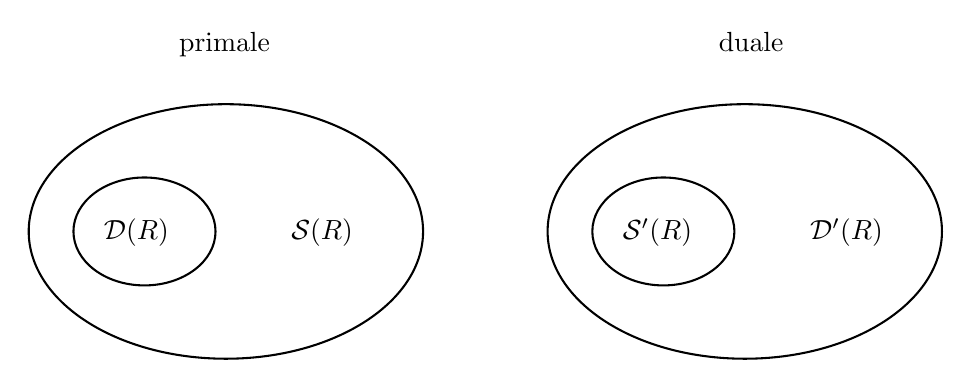
\begin{tikzpicture}[x=0.75pt,y=0.75pt,yscale=-1,xscale=1]
	%uncomment if require: \path (0,181); %set diagram left start at 0, and has height of 181

	%Shape: Ellipse [id:dp7503563455876929] 
	\draw   (80,108.68) .. controls (80,74.82) and (122.53,47.36) .. (175,47.36) .. controls (227.47,47.36) and (270,74.82) .. (270,108.68) .. controls (270,142.55) and (227.47,170) .. (175,170) .. controls (122.53,170) and (80,142.55) .. (80,108.68) -- cycle ;
	%Shape: Ellipse [id:dp5108599722199094] 
	\draw   (101.55,108.68) .. controls (101.55,94.32) and (116.87,82.68) .. (135.77,82.68) .. controls (154.68,82.68) and (170,94.32) .. (170,108.68) .. controls (170,123.04) and (154.68,134.68) .. (135.77,134.68) .. controls (116.87,134.68) and (101.55,123.04) .. (101.55,108.68) -- cycle ;
	%Shape: Ellipse [id:dp5851131130928555] 
	\draw   (330,108.68) .. controls (330,74.82) and (372.53,47.36) .. (425,47.36) .. controls (477.47,47.36) and (520,74.82) .. (520,108.68) .. controls (520,142.55) and (477.47,170) .. (425,170) .. controls (372.53,170) and (330,142.55) .. (330,108.68) -- cycle ;
	%Shape: Ellipse [id:dp4435469561254657] 
	\draw   (351.55,108.68) .. controls (351.55,94.32) and (366.87,82.68) .. (385.77,82.68) .. controls (404.68,82.68) and (420,94.32) .. (420,108.68) .. controls (420,123.04) and (404.68,134.68) .. (385.77,134.68) .. controls (366.87,134.68) and (351.55,123.04) .. (351.55,108.68) -- cycle ;

	% Text Node
	\draw (205,101.08) node [anchor=north west][inner sep=0.75pt]    {$\mathcal{S}(\mathbb{R})$};
	% Text Node
	\draw (114.77,101.08) node [anchor=north west][inner sep=0.75pt]    {$\mathcal{D}(\mathbb{R})$};
	% Text Node
	\draw (455,101.08) node [anchor=north west][inner sep=0.75pt]    {$\mathcal{D} '(\mathbb{R})$};
	% Text Node
	\draw (364.77,101.08) node [anchor=north west][inner sep=0.75pt]    {$\mathcal{S} '(\mathbb{R})$};
	% Text Node
	\draw (151,11) node [anchor=north west][inner sep=0.75pt]   [align=left] {primale};
	% Text Node
	\draw (411,11) node [anchor=north west][inner sep=0.75pt]   [align=left] {duale};


	\end{tikzpicture}
\end{figure}
\FloatBarrier
Questa riduzione dello spazio, è una riduzione stretta, cioè perdiamo alcuni elementi, vediamo un esempio.
\begin{equation*}
u=e^{x^{2}} \in L^{1}_{\mathrm{loc}} \ \ \Rightarrow \ \ \text{c'è una distribuzione associata}
\end{equation*}
tuttavia se consideriamo come funzione test una funzione di $\mathcal{S}(\mathbb{R})$ $\varphi =e^{-x^{2}}$
\begin{equation*}
( u,\varphi ) =\int _{\mathbb{R}} u\varphi dx=\int _{\mathbb{R}} dx=+\infty \ \ \Rightarrow \ \ \text{non è temperata}
\end{equation*}
\begin{definition}
[Convergenza di distribuzioni temperate] Sia $u_{n}$ una successione in $\{u_{n}\} \subset \mathcal{S} '(\mathbb{R})$. Diciamo che $u_{n}\rightarrow u\in \mathcal{S} '(\mathbb{R})$ se per ogni funzione test a decrescita rapida $\varphi \in \mathcal{S}(\mathbb{R})$, si ha $( u_{n} ,\varphi )\rightarrow ( u,\varphi )$.
\end{definition}
La definizione di derivata è la stessa.

Ora chiediamoci, se consideriamo una funzione $u\in L^{1}_{\mathrm{loc}}$, possiamo dire che vi è associata una distribuzione temperata? Abbiamo questo risultato.
\begin{theorem}
Se $\exists n\in \mathbb{N}$ tale che $( 1+| x| )^{-n} u( x) \in L^{1}(\mathbb{R})$ allora esiste una distribuzione temperata associata $u\in \mathcal{S} '(\mathbb{R})$.
\end{theorem}
\begin{theorem}
Se $u\in L^{p}(\mathbb{R})$ per un qualsiasi $p\in [ 1,+\infty ]$ allora esiste una distribuzione temperata associata $u\in \mathcal{S} '(\mathbb{R})$.
\end{theorem}
\chapter{Trasformate integrali}
\section{Introduzione}

È la versione \textit{continua} della serie di Fourier. Vedremo tutto sulla retta reale, ma si può applicare anche in $\mathbb{R}^{n}$. Consideriamo $\mathcal{D}(\mathbb{R}) \subset L^{p}(\mathbb{R}) \ \ \forall p\in [ 1,+\infty ]$, questa inclusione è densa $\forall p< +\infty $ (escluso).
\begin{definition}
[Inclusione densa] Dire che l'inclusione è densa significa dire che $\forall p< +\infty ,\forall f\in L^{p}(\mathbb{R})$ esiste $\varphi _{n} \in \mathcal{D}(\mathbb{R})$ tale che $\varphi _{n}\rightarrow f$ in senso $L^{p}$, cioè $\Vert \varphi _{n} -f\Vert _{L^{p}}\rightarrow 0$.
\end{definition}
Posso \textit{approssimare} ogni funzione in $L^{p}$ con $p< +\infty $ (funzioni anche molto irregolari e discontinue) con funzioni di $\mathcal{D}(\mathbb{R})$ (funzioni molto regolari e con cui è più semplice fare i conti), nel senso della norma ovviamente.



Introduciamo lo spazio
\begin{equation*}
\boxed{C^{0}_{0}(\mathbb{R}) =\left\{f\in C^{0}(\mathbb{R}) ,\lim _{x\rightarrow \pm \infty } f( x) =0\right\}} \subset L^{\infty }(\mathbb{R})
\end{equation*}
Le funzioni in $C^{0}_{0}(\mathbb{R})$ sono automaticamente limitate, quindi contenute nello spazio $L^{\infty }(\mathbb{R})$ delle funzioni \textit{essenzialmente} limitate. 	Questa inclusione \textbf{non} è densa.

Sia $f\in L^{1}(\mathbb{R})$ definiamo la funzione traslata
\begin{equation*}
f_{y}( x) =f( x-y)
\end{equation*}
\begin{theorem}
Sia $f\in L^{1}(\mathbb{R})$, allora
\begin{equation*}
\lim\limits _{y\rightarrow 0}\Vert f_{y} -f\Vert _{L^{1}} =0
\end{equation*}
\end{theorem}
\textit{Dimostrazione.}

È basata sulla densità a cui abbiamo accennato. Sia $\varepsilon  >0$, $\exists \varphi \in \mathcal{D}(\mathbb{R})$ tale che $\Vert f-\varphi \Vert < \varepsilon $. Se trasliamo una funzione, essa non cambia di norma $\Rightarrow \ \Vert f_{y} -\varphi _{y}\Vert < \varepsilon $. Chiamiamo $K$ un certo insieme che contiene sia il supporto di $\varphi $ che della sua traslata $\varphi _{y}$, per un certo $y$ sufficientemente piccolo. Allora\footnote{Teorema di Heine-Cantor. Una funzione continua su un compatto è uniformemente continua.} la funzione $\varphi $ è uniformemente continua, cioè
\begin{gather*}
\forall \varepsilon  >0\ \ \exists \delta \ \ | \varphi ( x) -\varphi ( y)| < \varepsilon \ \ \text{purché} \ | x-y| < \delta \\
\Updownarrow \\
\forall \varepsilon  >0\ \ \exists \delta \ \ | \varphi ( x-y) -\varphi ( x)| < \varepsilon \ \ \text{purché} \ | y| < \delta 
\end{gather*}
il delta che otteniamo \textit{non} dipende dal punto.

Dall'uniforme continuità deduciamo
\begin{equation*}
\Vert \varphi _{y} -\varphi \Vert =\int _{K}| \varphi ( x-y) -\varphi ( x)| dx< \varepsilon | K| 
\end{equation*}
Veniamo ora a
\begin{align*}
\Vert f_{y} -f\Vert  & =\Vert ( f_{y} -\varphi _{y}) +( \varphi _{y} -\varphi ) +( \varphi -f)\Vert \\
 & \leqslant \Vert f_{y} -\varphi _{y}\Vert +\Vert \varphi _{y} -\varphi \Vert +\Vert \varphi -f\Vert \\
 & < \varepsilon +\varepsilon | K| +\varepsilon \\
 & =\varepsilon ( 2+| K| )
\end{align*}
dove $( 2+| K| )$ è costante e $\varepsilon $ è arbitrario, cioè $\Vert f_{y} -f\Vert $ è tanto piccola quanto vogliamo.
\begin{equation*}
\qed 
\end{equation*}

Prima di procedere riassumiamo brevemente le inclusioni fra gli spazi che abbiamo visto

\begin{center}

\begin{tabular}{lc}
$\mathcal{D}(\mathbb{R}) \subset L^{p}(\mathbb{R})$ & densa $\forall p< +\infty $ \\
$\mathcal{D}(\mathbb{R}) \subset L^{p}(\mathbb{R})$ & densa $\forall p< +\infty $ \\
$\mathcal{D}(\mathbb{R}) \subset \mathcal{S}(\mathbb{R})$ & standard \\
$\mathcal{S} '(\mathbb{R}) \subset \mathcal{D} '(\mathbb{R})$ & standard \\
$C^{0}_{0}(\mathbb{R}) \subset L^{\infty }(\mathbb{R})$ & standard \\

\end{tabular}
\end{center}

\section{Trasformata di Fourier}

I numeri complessi entrano necessariamente nella trasformata di Fourier, quindi considereremo sempre funzioni $f:\mathbb{R}\rightarrow \mathbb{C}$.

Consideriamo $f\in L^{1}(\mathbb{R})$, definiamo \textbf{trasformata di Fourier} della funzione $f$
\begin{equation*}
\boxed{\hat{f}( z) =\int _{\mathbb{R}} e^{-izx} f( x) dx} \ \ \ \ f\in L^{1}(\mathbb{R})
\end{equation*}
Ci ricordiamo che i coefficienti di Fourier erano
\begin{equation*}
c_{n} =\frac{1}{\pi }\int ^{\pi }_{-\pi } e^{-inx} f( x) dx
\end{equation*}
È corretta la definizione?
\begin{equation*}
| f( x)| =\left| e^{-ixz} f( x)\right| 
\end{equation*}
ma $f$, e quindi anche $| f| $, è integrabile secondo Lebesgue, quindi anche il secondo membro è integrabile e convergente. Ha senso dare questa definizione! Vediamo di capire le proprietà, riassunte nel teorema fondamentale.
\begin{theorem}
[di Riemann-Lebesgue] Sia $f\in L^{1}(\mathbb{R})$, allora
\begin{equation*}
\boxed{\hat{f} \in C^{0}_{0}(\mathbb{R})} \ \ \ \ \boxed{\Vert \hat{f}\Vert _{\infty } \leqslant \Vert f\Vert _{L^{1}}}
\end{equation*}
\end{theorem}
La trasformata ha proprietà molto diverse e molto più regolari della $f$, che è banalmente integrabile, sta in uno spazio compeltamente diverso.

\textit{Dimostrazione.}

\textit{Continuità.}

Sia $z_{n}\rightarrow z\in \mathbb{R}$
\begin{equation*}
\lim\limits _{n\rightarrow +\infty }\hat{f}( z_{n}) =\lim\limits _{n\rightarrow +\infty }\int _{\mathbb{R}} e^{-iz_{n} x} f( x) dx
\end{equation*}
Notiamo che abbiamo la convergenza puntuale, quasi $\forall x$. Se usassimo l'integrale di Riemann non avremmo questo risultato, con Lebesgue, sì, usando la convergenza dominata.
\begin{equation*}
g_{n}\rightarrow g\ \text{q.o.} ,\ \exists h\in L^{1} ,\ | g_{n}| \leqslant h\ \forall n\ \ \Rightarrow \ \ \lim\limits _{n\rightarrow +\infty }\int g_{n} =\int \lim\limits _{n\rightarrow +\infty } g_{n}
\end{equation*}
qui possiamo maggiorare
\begin{equation*}
\underbrace{\left| e^{-iz_{n} x} f( x)\right| }_{| g_{n}| } \leqslant \underbrace{| f( x)| }_{h} \in L^{1}
\end{equation*}
quindi
\begin{equation*}
\lim\limits _{n\rightarrow +\infty }\int _{\mathbb{R}} e^{-iz_{n} x} f( x) dx=\int _{\mathbb{R}}\lim\limits _{n\rightarrow +\infty } e^{-iz_{n} x} f( x) dx=\int _{\mathbb{R}} e^{-izx} f( x) dx=\hat{f}( z)
\end{equation*}
\textit{Disuguaglianza delle norme.}

Chiaramente poi possiamo scrivere
\begin{equation*}
\Vert \hat{f}\Vert _{\infty } =| \hat{f}( z)| =\left| \int _{\mathbb{R}} e^{-ixz} f( x) dx\right| \leqslant \int _{\mathbb{R}}\left| e^{-ixz} f( x)\right| dx\leqslant \int _{\mathbb{R}}| f( x)| dx=\Vert f\Vert _{L^{1}}
\end{equation*}
\textit{Ultima parte.}

Ci resta da far vedere che
\begin{equation*}
\lim\limits _{z\rightarrow \pm \infty }\hat{f}( z) =0
\end{equation*}
Ricordiamo che $-1=e^{i\pi }$, scriviamo
\begin{equation*}
\hat{f}( z) =-e^{i\pi }\int _{\mathbb{R}} e^{-ixz} f( x) dx=-\int _{\mathbb{R}} e^{-i( xz-\pi )} f( x) dx=-\int _{\mathbb{R}} e^{-iz\left( x-\frac{\pi }{z}\right)} f( x) dx
\end{equation*}
cambiamo la variabile e ricordiamo che l'integrale è in $dx$
\begin{equation*}
x'=x-\frac{\pi }{z}
\end{equation*}
allora
\begin{equation*}
-\int _{\mathbb{R}} e^{-iz\left( x-\frac{\pi }{z}\right)} f( x) dx=-\int _{\mathbb{R}} e^{-izx'} f\left( x'+\frac{\pi }{z}\right) dx'=-\int _{\mathbb{R}} e^{-izx} f\left( x+\frac{\pi }{z}\right) dx
\end{equation*}
Scriviamo ora il doppio di $\hat{f}$
\begin{align*}
2\hat{f}( z) & =\int _{\mathbb{R}} e^{-ixz} f( x) dx-\int _{\mathbb{R}} e^{-izx} f\left( x+\frac{\pi }{z}\right) dx\\
 & =\int _{\mathbb{R}}\left[ e^{-ixz} f( x) -e^{-izx} f\left( x+\frac{\pi }{z}\right)\right] dx\\
 & =\int _{\mathbb{R}} e^{-ixz}\left[ f( x) -f\left( x+\frac{\pi }{z}\right)\right] dx
\end{align*}
passiamo al modulo
\begin{align*}
2| \hat{f}( z)|  & \leqslant \int _{\mathbb{R}}\left| e^{-ixz}\left[ f( x) -f\left( x+\frac{\pi }{z}\right)\right]\right| dx\\
 & =\int _{\mathbb{R}}\left| f( x) -f\left( x+\frac{\pi }{z}\right)\right| dx\\
 & =\Vert f-f_{-\pi /z}\Vert _{L^{1}}
\end{align*}
Quando $z\rightarrow \pm \infty $ la traslazione $-\pi /z\rightarrow 0$ e quindi, per quanto detto prima sulla traslazione di funzioni $L^{1}$ abbiamo $2| \hat{f}( z)| \rightarrow 0$.

\begin{equation*}
\qed 
\end{equation*}

Questo vuol dire che se chiamiamo
\begin{equation*}
\mathcal{F} :L^{1}(\mathbb{R})\rightarrow C^{0}_{0}(\mathbb{R})
\end{equation*}
abbiamo un operatore trasformata di Fourier che è, ovviamente, lineare, e, grazie alla disuguaglianza $\Vert \hat{f}\Vert _{\infty } \leqslant \Vert f\Vert _{L^{1}}$ anche limitata (e quindi equivalentemente anche continua, per quanto precedentemente). Cominciamo a verificare alcune proprietà.

Notazione: indichiamo con $\mathcal{F}( f( x) ,z) =\hat{f}( z)$ la trasformata di $f( x)$ scritta in funzione di $z$.
\begin{itemize}
\item Traslazione di $y\in \mathbb{R}$.\begin{equation*}
\begin{aligned}
\mathcal{F}( f( x-y) ,z) & =\int e^{-ixz} f( x-y) dx & x'=x-y\\
 & =\int e^{-ix'z-iyz} f( x') dx' & \\
 & =e^{-iyz}\int e^{-ixz} f( x) dx & \\
 & =e^{-iyz}\hat{f}( z) & \\
 & =e^{-iyz}\mathcal{F}( f( x) ,z) & 
\end{aligned}
\end{equation*}
\item Il contrario

\begin{equation*}
\begin{aligned}
\mathcal{F}\left( e^{iyx} f( x) ,z\right) & =\int e^{-ixz} e^{iyx} f( x) dx\\
 & =\int e^{-ix( z-y)} f( x) dx\\
 & =\hat{f}( z-y)\\
 & =\mathcal{F}( f( x) ,z-y)
\end{aligned}
\end{equation*}
\item $\mathcal{F}\left(\overline{f( x)} ,z\right) =\overline{\hat{f}( -z)}$
\item $f$ pari $\Rightarrow $ $\hat{f}$ pari
\item $f$ dispari $\Rightarrow $ $\hat{f}$ dispari
\item $f$ pari e reale $\Rightarrow $ $\hat{f}$ pari e reale
\item $f$ dispari e reale $\Rightarrow $ $\hat{f}$ dispari e immaginaria
\end{itemize}

Cerchiamo di capire se una trasformata di Fourier è derivabile, quindi anche $C^{1}$.
\begin{theorem}
[Derivata della trasformata] Sia $f\in L^{1}$, $g( x) =xf( x)$, $g\in L^{1}$. Allora $\hat{f} \in C^{1}$ e
\begin{equation*}
\hat{f} '( z) =-i\hat{g}( z) \ \ \text{cioè} \ \ \boxed{\frac{d^{n}}{dz^{n}}\mathcal{F}( f( x) ,z)= \mathcal{F}\left(( -ix)^{n} \cdotp f( x) ,z\right)}
\end{equation*}
\end{theorem}
Chiedere che anche $xf( x)$ stia in $L^{1}$ significa che la $f$ deve in qualche senso tendere a $0$ abbastanza rapidamente, vogliamo che l'integrale su $\mathbb{R}$ converga.

\textit{Dimostrazione.}

Calcoliamo il limite del rapporto incrementale
\begin{equation*}
\begin{aligned}
\lim\limits _{h\rightarrow 0}\frac{\hat{f}( z+h) -\hat{f}( z)}{h} & =\lim\limits _{h\rightarrow 0}\frac{1}{h}\left(\int e^{-ix( z+h)} f( x) dx-\int e^{-ixz} f( x) dx\right)\\
 & =\lim\limits _{h\rightarrow 0}\int e^{-ixz}\frac{e^{-ixh} -1}{h} f( x) dx\\
 & =\int e^{-ixz}( -ix) f( x) dx\\
 & =-i\mathcal{F}( xf( x) ,z)\\
 & =-i\hat{g}( z)
\end{aligned}
\end{equation*}
dove possiamo passare al limite sotto il segno di integrale perché in generale
\begin{equation*}
\left| e^{i\lambda } -1\right| \leqslant | \lambda | \ \ \lambda \in \mathbb{R} \ \ \ \ \ \ \ \ \lambda =-xh\ \ \Rightarrow \ \ \text{l'integrale converge per conv. dom.}\qed 
\end{equation*}
\begin{theorem}
[Trasformata della derivata] Sia $f\in L^{1} \cap C^{1}$, $f'\in L^{1}$.
\begin{equation*}
\boxed{\mathcal{F}\left(\frac{d^{n}}{dx^{n}} f( x) ,z\right) =( iz)^{n} \cdotp \mathcal{F}( f( x) ,z)}
\end{equation*}
\end{theorem}
Tutto questo è vero purché le cose scritte abbiano senso, da cui le ipotesi.
\section{Trasformazione inversa}
\begin{theorem}
Sia $f\in L^{1}$ e tale che $\hat{f} \in L^{1}$. Allora $f\in C^{0}_{0}$ e
\begin{equation*}
\boxed{f( x) =\frac{1}{2\pi }\int e^{ixz}\hat{f}( z) dz}
\end{equation*}
\end{theorem}
Perché le richieste sugli spazi di appartenenza? Supponiamo che questa sia l'antitrasformata, ha senso? È corretta? C'è in generale questo problema
\begin{equation*}
\begin{array}{ c c c }
f & \rightarrow  & \hat{f}\\
\in L^{1} &  & \in C^{0}_{0}
\end{array} \ \ \ \ \ \ \ \ \ \ \ \ \begin{array}{ c c c }
\hat{f} & \rightarrow  & f\\
\in L^{1} &  & \in C^{0}_{0}
\end{array}
\end{equation*}
La trasformata di Fourier non è simmetrica, lavora su spazi diversi. Se vogliamo che sia simmetrica nel senso che mandi uno spazio nello stesso spazio e ci permetta di tornare indietro possiamo farlo prendendo uno spazio un po' strano: $L^{1} \cap C^{0}_{0}$, vale infatti (non dimostriamo)
\begin{equation*}
\mathcal{F} :L^{1} \cap C^{0}_{0}\rightarrow L^{1} \cap C^{0}_{0}
\end{equation*}
\textbf{Problema!} Lo spazio $L^{1} \cap C^{0}_{0}$ non è uno spazio di Banach, non è completo né rispetto alla norma $L^{1}$ né rispetto alla norma $L^{\infty }$. Cercheremo ora di estendere la definizione allo spazio $L^{2}$, che oltre a essere di Banach è anche di Hilbert
\begin{equation*}
\mathcal{F} :L^{2}\rightarrow L^{2}
\end{equation*}
\section{Convoluzione}
\begin{theorem}
Siano $u,v\in L^{1}(\mathbb{R})$. Allora la funzione
\begin{equation*}
\boxed{( u*v)( x) =\int _{\mathbb{R}} u( x-t) v( t) dt}
\end{equation*}
è definita per \underline{quasi ogni} $x\in \mathbb{R}$, $( u*v) \in L^{1}$ e inoltre, stando in $L^{1}$, avrà una norma $\Vert u*v\Vert _{L^{1}} \leqslant \Vert u\Vert _{L^{1}}\Vert v\Vert _{L^{1}}$.
\end{theorem}
Discende direttamente dal teorema di Fubini.
\begin{itemize}
\item È simmetrica

\begin{equation*}
\begin{aligned}
( u*v)( x) & =\int _{\mathbb{R}} u( x-t) v( t) dt & t'=x-t\\
 & =\int _{\mathbb{R}} u( t') v( x-t') dt' & \\
 & =( v*u)( x) & 
\end{aligned}
\end{equation*}
\item È associativa\begin{align*}
( u*v) *w & =u*( v*w)
\end{align*}
\item Supponiamo di avere

\begin{gather*}
u( x) =\begin{cases}
n & x\in \left[ 0,\frac{1}{n}\right]\\
0 & \text{altrove}
\end{cases} \ \ \ \ \Vert u\Vert =1\\
( u*v)( x) =\int _{\mathbb{R}} u( x-t) v( t) dt=n\int ^{x}_{x-\frac{1}{n}} v( t) dt
\end{gather*}

è la media della funzione $v$ calcolata in un intorno di $x$. L'effetto della convoluzione è in qualche modo di smussare il valore della funzione $v$, in ogni punto sostutiamo la media in un suo intorno.
\end{itemize}

Qual è il legame con la trasformata di Fourier? Siano $u,v\in L^{1}$, calcoliamo la trasformata di $u*v$, dato che sta in $L^{1}$
\begin{align*}
\mathcal{F}( u*v,z) & =\int e^{-ixz}\left[\int u( x-t) v( t) dt\right] dx\\
 & =\int e^{-iz( x-t)} e^{-izt} u( x-t) v( t) dtdx\\
 & =\int e^{-izt} v( t)\left[\int e^{-iz( x-t)} u( x-t) dx\right] dt
\end{align*}
con un cambio di variabile $x'=x-t$
\begin{align*}
\int e^{-izt} v( t)\left[\int e^{-iz( x-t)} u( x-t) dx\right] dt & =\int e^{-izt} v( t)\left[\int e^{-izx'} u( x') dx'\right] dt\\
 & =\hat{u}( z)\hat{v}( z)
\end{align*}
Vale anche il contrario
\begin{equation*}
\mathcal{F}^{-1}(\hat{u} *\hat{v} ,x) =u( x) v( x)
\end{equation*}
\section{Estensione della trasformata di Fourier}

Introduzione
\begin{itemize}
\item Ci serviremo della proprietà che $\mathcal{D}(\mathbb{R}) \subset \mathcal{S}(\mathbb{R}) \subset L^{p}(\mathbb{R})$ è un'inclusione densa per ogni $p< +\infty $
\item Lavoriamo in $\boxed{\mathcal{S}(\mathbb{R})}$ per estendere la trasformata perché la trasformata di una funzione in $\mathcal{S}(\mathbb{R})$ è ancora una funzione in $\mathcal{S}(\mathbb{R})$, mentre la trasformata di una funzione in $\mathcal{D}(\mathbb{R})$ è ancora $C^{\infty }$, ma non più necessariamente a supporto compatto.
\end{itemize}
\subsection{Allo spazio di funzioni a descrescenza rapida}
\begin{theorem}
La trasformata agisce su
\begin{equation*}
\mathcal{F} :\mathcal{S}(\mathbb{R})\rightarrow \mathcal{S}(\mathbb{R})
\end{equation*}
\end{theorem}
\textit{Dimostrazione.}

Lo spazio di partenza ha senso essendo densamente incluso in $L^{p}(\mathbb{R}) ,p=1$.

Sia $u\in S(\mathbb{R})$, consideriamo $v( x) =x^{N} u( x) \in \mathcal{S}(\mathbb{R}) \subset L^{1}(\mathbb{R})$.
\begin{itemize}
\item Trasformata della derivata di $v$ $M$ volte\begin{equation*}
\mathcal{F}\left( v^{( M)} ,z\right) =( iz)^{M}\hat{v} \in L^{\infty }(\mathbb{R})
\end{equation*}

dato che $v$ sta in $L^{1}$, $\hat{v}$ sta in $C^{0}_{0}$, quindi la quantità $( iz)^{M}\hat{v}$ è limitata
\item Derivata della trasformata di $u$ $N$ volte\begin{equation*}
\hat{u}^{( N)} =( -i)^{N}\hat{v}
\end{equation*}

moltiplichiamola per $z^{M}$, il termine che otteniamo a destra abbiamo appena fatto vedere che, a meno di coefficienti $i$ opportunamente elevati, è limitato\begin{equation*}
z^{M}\hat{u}^{( N)} =z^{M}( -i)^{N}\hat{v} \ \ \boxed{\in L^{\infty }(\mathbb{R})} \ \ \forall N,M\geqslant 0
\end{equation*}ma questa è proprio la definizione di funzione a descrescenza rapida, quindi $\hat{u} \in \mathcal{S}(\mathbb{R})$ e abbiamo dimostrato la tesi.\begin{equation*}
\end{equation*}
\end{itemize}
\subsection{Allo spazio $L^{2}$}

Vogliamo mostrare che
\begin{equation*}
\mathcal{F} :L^{2}(\mathbb{R})\rightarrow L^{2}(\mathbb{R})
\end{equation*}
Non possiamo definirla in $L^{2}$ come $\int e^{-ixz} u( x) dx$ perché se $u\in L^{2}$ non abbiamo nessuna garanzia che la funzione sia integrabile. Partiamo definendo la trasformata in $L^{1}(\mathbb{R}) \cap L^{2}(\mathbb{R})$.
\begin{theorem}
[di Plancherel] Sia $u\in L^{1}(\mathbb{R}) \cap L^{2}(\mathbb{R})$, allora
\begin{equation*}
\boxed{\Vert \hat{u}\Vert _{L^{2}} =\sqrt{2\pi }\Vert u\Vert _{L^{2}}} \ \ \text{quindi} \ \ \boxed{\hat{u} \in L^{2}(\mathbb{R})}
\end{equation*}
\end{theorem}
\textit{Dimostrazione.}
\begin{itemize}
\item \textit{Dimostrazione nel caso di }$u\in \mathcal{S}(\mathbb{R})$

Dato che $u\in \mathcal{S}(\mathbb{R})$, allora $u\in L^{2}$. Ci serve partira da $u\in \mathcal{S}(\mathbb{R})$ per poter usare correttamente il risultato di inversione, in accordo a quanto appena detto sull'estensione a $\mathcal{F} :\mathcal{S}(\mathbb{R})\rightarrow \mathcal{S}(\mathbb{R})$.

\begin{equation*}
\begin{aligned}
\Vert u\Vert ^{2}_{L^{2}} & =\int | u( x)| ^{2} dx=\int \overline{u( x)} u( x) dx & \text{essendo} \ u\in L^{2}(\mathbb{R})\\
u( x) & =\frac{1}{2\pi }\int e^{ixz}\hat{u}( z) dz & \text{essendo} \ u\in \mathcal{S}(\mathbb{R})
\end{aligned}
\end{equation*}

Sostituiamo

\begin{equation*}
\begin{aligned}
\Vert u\Vert ^{2}_{L^{2}} & =\frac{1}{2\pi }\int \overline{u( x)}\int e^{ixz}\hat{u}( z) dzdx & \\
 & =\frac{1}{2\pi }\int \hat{u}( z)\int \overline{e^{-ixz} u( x)} dxdz & \text{(Fubini)}\\
 & =\frac{1}{2\pi }\int \hat{u}( z)\overline{\hat{u}( z)} dz & \\
 & =\frac{1}{2\pi }\Vert \hat{u}\Vert ^{2}_{L^{2}} \ \ \Rightarrow \ \ \Vert \hat{u}\Vert _{L^{2}} =\sqrt{2\pi }\Vert u\Vert _{L^{2}} & 
\end{aligned}
\end{equation*}

Stando $u\in L^{2}$, ciò che sta a destra dell'uguale è un numero finito, quindi anche ciò che è a sinistra, quindi $\hat{u}$ appartiene ad $L^{2}$.
\item \textit{Estensione a }$u\in L^{2}(\mathbb{R})$

Per \textbf{densità} dell'inclusione $\mathcal{S}(\mathbb{R}) \subset L^{2}(\mathbb{R})$,
\begin{itemize}
\item posso costruire una successione approssimante\begin{equation*}
L^{2}(\mathbb{R}) \supset \mathcal{S}(\mathbb{R}) \ni u_{n}\xrightarrow{L^{2}} u\in L^{2}(\mathbb{R})
\end{equation*}
\item posso fare le trasformate $\widehat{u_{n}}$ dato che $u_{n} \in \mathcal{S}(\mathbb{R})$
\item per l'uguaglianza delle norme appena trovata, valida appunto per $u_{n} \in \mathcal{S}(\mathbb{R})$\begin{equation*}
\Vert u_{n} -u_{m}\Vert _{L^{2}} =\Vert \hat{u}_{n} -\hat{u}_{m}\Vert _{L^{2}}\frac{1}{\sqrt{2\pi }}
\end{equation*}

Grazie alla completezza dello spazio $L^{2}$, se $u_{n}$ converge, è di Cauchy, allora lo è anche la sua trasformata, allora anche lei converge. Definisco $\hat{u}$ il limite della successione $\widehat{u_{n}}\xrightarrow{L^{2}}\hat{u}$, abbiamo trovato la trasformata $\mathcal{F} :L^{2}\rightarrow L^{2}$.
\end{itemize}
\item Con questo ragionamento potremmo anche dedurre che

\begin{equation*}
( u,v) =\frac{1}{2\pi }(\hat{u} ,\hat{v}) \ \ \ \ \text{(si mantiene l'ortogonalità)}\qed 
\end{equation*}
\end{itemize}
\section{Trasformata di Fourier di una distribuzione temperata}

Ci manca solo la trasformata di Fourier di una distribuzione temperata, consideriamo quindi $S'(\mathbb{R})$. Vogliamo mostrare che
\begin{equation*}
\mathcal{F} :S'(\mathbb{R})\rightarrow S'(\mathbb{R})
\end{equation*}
Ricordiamo che
\begin{equation*}
( u',\varphi ) =-( u,\varphi ')
\end{equation*}
Supponiamo che $u$ sia una distribuzione temperata $u\in \mathcal{S} '(\mathbb{R})$, vorremmo che $\hat{u} \in \mathcal{S} '(\mathbb{R})$. Definiamo senza nessuno sforzo
\begin{equation*}
\boxed{(\hat{u} ,\varphi ) =( u,\hat{\varphi })} \ \ \ \ \varphi \in \mathcal{S}(\mathbb{R})
\end{equation*}
dato che se $\varphi \in \mathcal{S}(\mathbb{R})$ allora $\hat{\varphi } \in \mathcal{S}(\mathbb{R})$.
\begin{theorem}
La trasformata di Fourier $\mathcal{F} :\mathcal{S} '(\mathbb{R})\rightarrow \mathcal{S} '(\mathbb{R})$ è un'applicazione

lineare biunivoca e continua.
\end{theorem}
\textit{Dimostrazione.}
\begin{itemize}
\item È effettivamente un funzionale \textbf{lineare} dalla definizione
\item \textbf{Continuo} grazie alla (non dimostrata) continuità della trasformata di Fourier delle funzioni in $\mathcal{S}(\mathbb{R})$.\begin{equation*}
(\hat{u} ,\varphi _{n}) =\left( u,\widehat{\varphi _{n}}\right)\rightarrow ( u,\hat{\varphi }) =(\hat{u} ,\varphi )
\end{equation*}
\item \textbf{Suriettiva.}\begin{equation*}
\begin{array}{ c c c }
\mathcal{F} :\mathcal{S} '(\mathbb{R}) & \rightarrow  & \mathcal{S} '(\mathbb{R})\\
u &  & \hat{u} =v
\end{array}
\end{equation*}

Data una distribuzione temperata $v\in \mathcal{S} '(\mathbb{R})$ tale che $v=\hat{u}$ dobbiamo trovare $u\in \mathcal{S} '(\mathbb{R})$. Diciamo che $u=\mathcal{F}^{-1}( v)$, e infatti\begin{equation*}
(\hat{u} ,\varphi ) =( u,\hat{\varphi }) =\left(\mathcal{F}^{-1}( v) ,\hat{\varphi }\right) =\left( v,\mathcal{F}^{-1}(\hat{\varphi })\right) =( v,\varphi ) \ \ \forall \varphi 
\end{equation*}
\item \textbf{Iniettiva}.

Dobbiamo far vedere che se abbiamo $u_{1} ,u_{2} \in \mathcal{S} '(\mathbb{R})$ e $\hat{u}_{1} =\hat{u}_{2}$ allora $u_{1} =u_{2}$. Prendiamo una nuova funzione test $\psi $ tale che $\hat{\psi } =\varphi $.\begin{equation*}
( u_{1} ,\varphi ) =( u_{1} ,\hat{\psi }) =(\hat{u}_{1} ,\psi ) =(\hat{u}_{2} ,\psi ) =( u_{2} ,\hat{\psi }) =( u_{2} ,\varphi )\qed 
\end{equation*}
\end{itemize}
\textit{Esempio.}

Calcoliamo la trasformata di Fourier di una costante, cioè una funzione $L^{1}_{\mathrm{loc}}$ a cui quindi è associata una distribuzione temperata\footnote{Si noti che in testi differenti si potrebbe trovare un risultato diverso in base a come si è definita la trasformata di Fourier. Non tutti, infatti, sono d'accordo sull'uso della costante $2\pi $ tra la trasformazione diretta e quella inversa.}
\begin{equation*}
\mathcal{F}^{-1}\{\delta _{0}( \xi )\} =\frac{1}{2\pi }\int _{\mathbb{R}} e^{i\xi x} \delta _{0}( \xi ) d\xi =\frac{1}{2\pi } \langle \delta _{0}( \xi ) ,e^{i\xi x} \rangle =\frac{1}{2\pi }
\end{equation*}
allora
\begin{equation*}
\mathcal{F}\left\{\frac{1}{2\pi }\right\} =\delta _{0}( \xi ) \ \ \Rightarrow \ \ \boxed{\mathcal{F}\{1\} =2\pi \delta _{0}( \xi )}
\end{equation*}
\section{Trasformata di Laplace}

È parente stretta della trasformata di Fourier, solo che Fourier si riferisce a tutto $\mathbb{R}^{n}$, Laplace su funzioni definite su una semiretta. Questa differenza si riflette sul loro impiego per le equazioni differenziali.

Cosa deve avere una funzione $u:\mathbb{R}\rightarrow \mathbb{R}$ affinché sia Laplace-trasformabile o $\mathcal{L}$-trasformabile?
\begin{itemize}
\item $\mathrm{supp}( u) \subset [ 0,+\infty )$

A questo proposito ricordiamo la funzione di Heaviside, che sarà utile, in quanto non trasformeremo mai $\sin x$, piuttosto trasformeremo $H( x)\sin x$, anche se talvolta sorvoleremo su questa cosa dandola per scontata\begin{equation*}
H( x) =\begin{cases}
1, & \text{se} \ x\geqslant 0\\
0, & \text{se} \ x< 0
\end{cases}
\end{equation*}
\item $u\in L^{1}_{\mathrm{loc}}$
\item $\exists \lambda \in \mathbb{R}$ tale che $e^{-\lambda x} u( x) \in L^{1}(\mathbb{R})$

Chiamiamo $\lambda ( u)$ l'estremo inferiore di questi $\lambda $
\end{itemize}
\begin{definition}
[Trasformata di Laplace] Definiamo
\begin{equation*}
\boxed{\mathcal{L}( u( x) ,s) =\int ^{+\infty }_{0} e^{-sx} u( x) dx} \ \ \ \ s\in \mathbb{C}
\end{equation*}
dove
\begin{equation*}
e^{-sx} =e^{-s_{R} x} e^{-is_{I} x}
\end{equation*}
Questo integrale ha senso purché $e^{-\lambda x} u( x) \in L^{1}(\mathbb{R})$, cioè $\mathrm{Re}( s)  >\lambda ( u)$, che è quindi il dominio della trasformata, mentre Fourier aveva senso sempre.
\end{definition}
\textbf{Proprietà}
\begin{itemize}
\item Linearità $\boxed{\mathcal{L}( \alpha u( x) +\beta v( x) ,s) =\alpha \mathcal{L}( u( x) ,s) +\beta \mathcal{L}( v( x) ,s)}$

Attenzione, dobbiamo intersecare i due domini\begin{equation*}
\boxed{\mathrm{Re}( s)  >\max( \lambda ( u) ,\lambda ( v))}
\end{equation*}
\item $\boxed{\lim\limits _{\mathrm{Re}( s)\rightarrow +\infty }\mathcal{L}( u( x) ,s) =0}$

\textit{Dimostrazione.}\begin{equation*}
\lim\limits _{\mathrm{Re}( s)\rightarrow +\infty }\mathcal{L}( u( x) ,s) =\lim\limits _{\mathrm{Re}( s)\rightarrow +\infty }\int ^{+\infty }_{0} e^{-s_{R} x} e^{-is_{I} x} u( x) dx
\end{equation*}

possiamo portare il limite dentro per convergenza dominata, purché $\mathrm{Re}( s)  >\lambda ( u)$ possiamo trovare una funzione che la domini\begin{equation*}
\lim\limits _{\mathrm{Re}( s)\rightarrow +\infty }\int ^{+\infty }_{0} e^{-s_{R} x} e^{-is_{I} x} u( x) dx=\int ^{+\infty }_{0}\lim\limits _{\mathrm{Re}( s)\rightarrow +\infty } e^{-s_{R} x} e^{-is_{I} x} u( x) dx=0
\end{equation*}
\item $\boxed{\mathcal{L}( u( x-x_{0}) ,s) =e^{-sx_{0}}\mathcal{L}( u( x) ,s)}$

Attenzione che essendo $\mathrm{supp}( u) \in [ 0,+\infty )$
\begin{itemize}
\item se $\boxed{x_{0}  >0}$ il supporto è ancora quello
\item se $x_{0} < 0$ il supporto potrebbe includere numeri negativi, quindi scartiamo questo caso
\end{itemize}

\textit{Dimostrazione.}\begin{equation*}
\begin{aligned}
\mathcal{L}( u( x-x_{0}) ,s) & =\int ^{+\infty }_{0} e^{-sx} u( x-x_{0}) dx & x'=x-x_{0}\\
 & =\int ^{+\infty }_{-x_{0}} e^{-s( x'+x_{0})} u( x') dx' & \\
 & =\int ^{+\infty }_{0} e^{-s( x'+x_{0})} u( x') dx' & \\
 & =e^{-sx_{0}}\mathcal{L}( u( x) ,s) & 
\end{aligned}
\end{equation*}
\item $\boxed{\mathcal{L}\left( e^{s_{0} x} u( x) ,s\right) =\mathcal{L}( u( x) ,s-s_{0})}$ $\boxed{\mathrm{Re}( s-s_{0})  >\lambda ( u)}$

\textit{Dimostrazione.}\begin{equation*}
\mathcal{L}\left( e^{s_{0} x} u( x) ,s\right) =\int ^{+\infty }_{0} e^{-x( s-s_{0})} u( x) dx=\mathcal{L}( u( x) ,s-s_{0})
\end{equation*}
\item $\boxed{\mathcal{L}( u( cx) ,s) =\frac{1}{c}\mathcal{L}\left( u( x) ,\frac{s}{c}\right)}$ $\boxed{c\in \mathbb{R} ,c >0}$

\textit{Dimostrazione.}\begin{equation*}
\begin{aligned}
\mathcal{L}( u( cx) ,s) & =\int ^{+\infty }_{0} e^{-sx} u( cx) dx & x'=cx\ \ \Rightarrow \ \ dx'=cdx\\
 & =\int ^{+\infty }_{0} e^{-s\frac{x'}{c}} u( x')\frac{1}{c} dx' & \\
 & =\frac{1}{c}\mathcal{L}\left( u( x) ,\frac{s}{c}\right) & 
\end{aligned}
\end{equation*}
\end{itemize}
\subsection{Trasformate di funzioni notevoli}
\begin{itemize}
\item Heaviside\begin{align*}
\mathcal{L}( H( x) ,s) & =\int ^{+\infty }_{0} e^{-sx} H( x) dx=\int ^{+\infty }_{0} e^{-sx} dx\\
 & =\left[ -\frac{e^{-sx}}{s}\right]^{+\infty }_{0} =\frac{1}{s} -\lim _{r\rightarrow +\infty }\frac{e^{-sr}}{s}\\
 & =\frac{1}{s} \ \ \ \ \text{purché} \ \mathrm{Re}( s)  >0
\end{align*}

il che ci dice anche che $\lambda ( H) =0$, confermato da\begin{equation*}
e^{-\lambda x} H( x) \in L^{1}(\mathbb{R}) \ \ \ \ \lambda  >0
\end{equation*}

Perché ci serve?\begin{equation*}
\mathcal{L}\left( e^{s_{0} x} H( x) ,s\right) =\mathcal{L}( H( x) ,s-s_{0}) =\frac{1}{s-s_{0}}
\end{equation*}
\item Seno e coseno\begin{align*}
\mathcal{L}(\cos( \omega x) H( x) ,s) & =\mathcal{L}\left(\frac{e^{i\omega x} +e^{-i\omega x}}{2} ,s\right)\\
 & =\frac{1}{2}\left(\frac{1}{s-i\omega x} +\frac{1}{s+i\omega x}\right) =\frac{1}{2}\frac{2s}{s^{2} +\omega ^{2}} =\frac{s}{s^{2} +\omega ^{2}}\\
\mathcal{L}(\sin( \omega x) H( x) ,s) & =\frac{\omega }{s^{2} +\omega ^{2}}
\end{align*}
\item Delta di Dirac \textit{trattandola come funzione}.\begin{align*}
\mathcal{L}( \delta _{0} ,s) & =\int ^{+\infty }_{0} e^{-sx} \delta _{0}( x) dx=1
\end{align*}

per capirlo meglio possiamo vedere la Delta come\begin{gather*}
\delta _{0} =\lim\limits _{\varepsilon \rightarrow 0} u_{\varepsilon }( x) \ \ \ \ u_{\varepsilon }( x) =\begin{cases}
\frac{1}{\varepsilon } , & x\in [ 0,\varepsilon ]\\
0, & \text{altrimenti}
\end{cases}\\
\mathcal{L}( u_{\varepsilon }( x) ,s) =\frac{1}{\varepsilon }\int ^{\varepsilon }_{0} e^{-sx} dx=e^{-sx_{\varepsilon }}\rightarrow 1\ \ x_{\varepsilon } \in ( 0,\varepsilon )
\end{gather*}
\end{itemize}
\begin{theorem}
[Derivata della trasformata] Sia $u$ una funzione $\mathcal{L}$-trasformabile.
\begin{equation*}
\boxed{\frac{d^{n}}{ds^{n}}\mathcal{L}( u( x) ,s) =(\mathcal{-1)^{n} L}\left( x^{n} u( x) ,s\right)} \ \ \ \ \forall s\ \text{tale che} \ \mathrm{Re}( s)  >\lambda ( u)
\end{equation*}
\end{theorem}
\textit{Dimostrazione.}
\begin{align*}
\lim\limits _{h\rightarrow 0}\frac{\mathcal{L}( u( x) ,s+h) -\mathcal{L}( u( x) ,s)}{h} & =\lim\limits _{h\rightarrow 0}\int ^{+\infty }_{0} e^{-sx}\frac{e^{-hx} -1}{h} u( x) dx\\
 & =\int ^{+\infty }_{0}\lim\limits _{h\rightarrow 0} e^{-sx}\textcolor[rgb]{0.82,0.01,0.11}{\frac{e^{-hx} -1}{-hx}}( -x) u( x) dx\\
 & =\int ^{+\infty }_{0} e^{-sx}( -x) u( x) dx\\
 & =-\mathcal{L}( xu( x) ,s)
\end{align*}
Possiamo passare al limite sotto il segno di integrale? Sì perché la quantità rossa è limitata, il resto è $L^{1}$.

È derivabile in un aperto in senso complesso, quindi la funzione trasformata di Laplace è olomorfa, quindi è anche $C^{\infty }$.
\begin{theorem}
[Trasformata della derivata] Sia $u$ una funzione $\mathcal{L}$-trasformabile e $u\in C^{1}([ 0,+\infty ))$. Chiamiamo $v( x)$ la derivata
\begin{equation*}
v( x) =\begin{cases}
u'( x) & x\geqslant 0\\
0 & x< 0
\end{cases}
\end{equation*}
dove $u'( x)$ è estesa per continuità nell'origine.

Sia quindi anche $v$ $\mathcal{L}$-trasformabile. Allora
\begin{equation*}
\boxed{\mathcal{L}( v( x) ,s) =s\mathcal{L}( u( x) ,s) -u( 0)}
\end{equation*}
attenzione che in realtà $u( 0)$ è il limite per $x\rightarrow 0^{+}$, dato che non è di solito continua nell'origine.

Inoltre
\begin{equation*}
\lim _{\mathrm{Re}( s)\rightarrow +\infty } s\mathcal{L}( u( x) ,s) =u( 0)
\end{equation*}
Se $v\in L^{1}$, allora $\lambda ( u) \leqslant 0$ e
\begin{equation*}
\lim\limits _{s\rightarrow 0,\ \mathrm{Re}( s)  >0} s\mathcal{L}( u( x) ,s) =\lim _{x\rightarrow +\infty } u( x)
\end{equation*}
\end{theorem}
\textit{Dimostrazione della prima parte.}
\begin{equation*}
\begin{aligned}
\mathcal{L}( u'( x) ,s) & =\int ^{+\infty }_{0} e^{-sx} u'( x) dx & \text{(per parti)}\\
 & =\left[ e^{-sx} u( x)\right]^{+\infty }_{0} -( -s)\int ^{+\infty }_{0} e^{-sx} u( x) dx & \\
 & =\lim _{x\rightarrow +\infty } e^{-sx} u( x) -u( 0) +s\mathcal{L}( u( x) ,s) & 
\end{aligned}
\end{equation*}
Notiamo che
\begin{equation*}
e^{-\lambda x} u( x) \in L^{1} \ \ \nRightarrow \ \ e^{-\lambda x} u( x)\rightarrow 0\ \text{per} \ x\rightarrow +\infty 
\end{equation*}
per esempio questa funzione non tende a $0$ pur essendo integrabile

\begin{figure}[htpb]
	\centering
	

	\tikzset{every picture/.style={line width=0.75pt}} %set default line width to 0.75pt        

	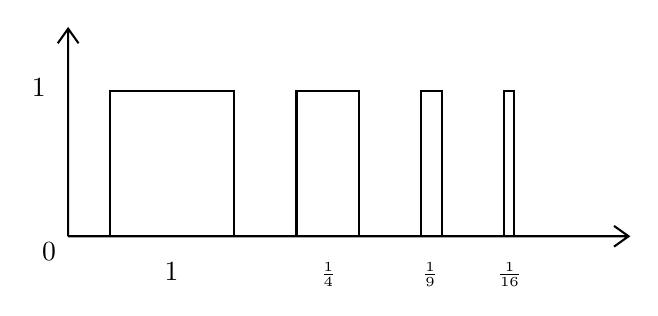
\begin{tikzpicture}[x=0.75pt,y=0.75pt,yscale=-1,xscale=1]
	%uncomment if require: \path (0,159); %set diagram left start at 0, and has height of 159

	%Shape: Axis 2D [id:dp9522434839194833] 
	\draw  (171,111) -- (441,111)(171,11) -- (171,111) -- cycle (434,106) -- (441,111) -- (434,116) (166,18) -- (171,11) -- (176,18)  ;
	%Shape: Rectangle [id:dp6209341938001463] 
	\draw   (191,41) -- (251,41) -- (251,111) -- (191,111) -- cycle ;
	%Shape: Rectangle [id:dp5551932751144555] 
	\draw   (281,41) -- (311,41) -- (311,111) -- (281,111) -- cycle ;
	%Shape: Rectangle [id:dp45095610787740714] 
	\draw   (341,41) -- (351,41) -- (351,111) -- (341,111) -- cycle ;
	%Shape: Rectangle [id:dp9386110377703627] 
	\draw   (381,41) -- (386,41) -- (386,111) -- (381,111) -- cycle ;

	% Text Node
	\draw (152,33.4) node [anchor=north west][inner sep=0.75pt]    {$1$};
	% Text Node
	\draw (291,122.4) node [anchor=north west][inner sep=0.75pt]  [font=\scriptsize]  {$\frac{1}{4}$};
	% Text Node
	\draw (216,122.4) node [anchor=north west][inner sep=0.75pt]    {$1$};
	% Text Node
	\draw (157,112.4) node [anchor=north west][inner sep=0.75pt]    {$0$};
	% Text Node
	\draw (340,122.4) node [anchor=north west][inner sep=0.75pt]  [font=\scriptsize]  {$\frac{1}{9}$};
	% Text Node
	\draw (376,122.4) node [anchor=north west][inner sep=0.75pt]  [font=\scriptsize]  {$\frac{1}{16}$};


	\end{tikzpicture}
\end{figure}
\FloatBarrier

\begin{equation*}
\int ^{+\infty }_{0} f( x) dx=\sum ^{\infty }_{n=1}\frac{1}{n^{2}} < +\infty \ \ \ \ \text{ma} \ f( x) \nrightarrow 0
\end{equation*}
Analizziamo bene però la nostra funzione, derivandola
\begin{equation*}
\frac{d}{dx}\left( e^{-\lambda x} u( x)\right) =\underbrace{-\lambda e^{-\lambda x} u( x)}_{\in L^{1}} +\underbrace{e^{-\lambda x} u'( x)}_{\in L^{1}} \in L^{1}
\end{equation*}
le due parti sono integrabili per ipotesi, grazie al fatto che anche $u'$ deve essere $\mathcal{L}$-trasformabile. Per il teoreoma del calcolo
\begin{equation*}
e^{-\lambda x} u( x) =u( 0) +\int ^{x}_{0}\frac{d}{dt}\left( e^{-\lambda t} u( t)\right) dt
\end{equation*}
il limite a destra esiste finito, allora esiste finito il limite di $e^{-\lambda x} u( x)$, ma se ammette limite deve necessariamente essere
\begin{gather*}
\lim _{x\rightarrow +\infty } e^{-sx} u( x) =0\\
\qed 
\end{gather*}
\subsection{Trasformazione inversa}

Se abbiamo $f( s) =\mathcal{L}( u( x) ,s)$ come troviamo $u( x) =\mathcal{L}^{-1}( f( s) ,s)$?

Scriviamo $s=a+ib$.
\begin{equation*}
f( a+ib) =\int ^{+\infty }_{0} e^{-ax} e^{-ibx} u( x) dx=\int _{\mathbb{R}} e^{-ax} e^{-ibx} u( x) dx=\mathcal{F}\left( e^{-ax} u( x) ,b\right)
\end{equation*}
Ma allora possiamo fare l'antitrasformata di Fourier!
\begin{equation*}
e^{-ax} u( x) =\frac{1}{2\pi }\int _{\mathbb{R}} f( a+ib) e^{ibx} db
\end{equation*}
allora
\begin{equation*}
\boxed{u( x) =\frac{1}{2\pi }\int _{\mathbb{R}} e^{( a+ib) x} f( a+ib) db} \ \ \ \ \forall a >\lambda ( u)
\end{equation*}
Questa è già una formula valida, ma possiamo chiamare, per $x$ fissato
\begin{equation*}
\Gamma _{x} =\{z\in \mathbb{C} ,z=x+iy,y\in \mathbb{R}\}
\end{equation*}

\begin{figure}[htpb]
	\centering
	\tikzset{every picture/.style={line width=0.75pt}} %set default line width to 0.75pt        

	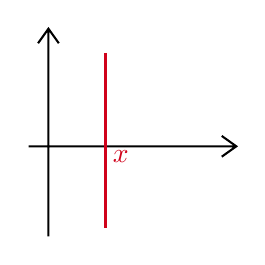
\begin{tikzpicture}[x=0.75pt,y=0.75pt,yscale=-1,xscale=1]
	%uncomment if require: \path (0,113); %set diagram left start at 0, and has height of 113

	%Shape: Axis 2D [id:dp6665420354493967] 
	\draw  (251,63.66) -- (351,63.66)(260.5,7) -- (260.5,107) (344,58.66) -- (351,63.66) -- (344,68.66) (255.5,14) -- (260.5,7) -- (265.5,14)  ;
	%Straight Lines [id:da4009061220418899] 
	\draw [color={rgb, 255:red, 208; green, 2; blue, 27 }  ,draw opacity=1 ]   (288,18.66) -- (288,103) ;

	% Text Node
	\draw (290,64.23) node [anchor=north west][inner sep=0.75pt]  [color={rgb, 255:red, 208; green, 2; blue, 27 }  ,opacity=1 ]  {$x$};


	\end{tikzpicture}
\end{figure}
\FloatBarrier

E possiamo allora scrivere l'antitrasformata come
\begin{equation*}
\boxed{u( x) =\frac{1}{2\pi }\int _{\Gamma _{x}} e^{zx} f( z) dz}
\end{equation*}
\section{Relazione con la convoluzione}

Ricordiamo la convoluzione di due funzioni $f,g\in L^{1}$
\begin{equation*}
( f*g)( x) =\int _{\mathbb{R}} f( x-t) g( t) dt
\end{equation*}
Con Fourier abbiamo, utile in entrambi i versi,
\begin{equation*}
\mathcal{F}( f*g,z) =\hat{f}( z)\hat{g}( z)
\end{equation*}
Per Laplace abbiamo le seguenti richieste sulle funzioni affinché siano $\mathcal{L}$-trasformabili
\begin{itemize}
\item $f,g\in L^{1}_{\mathrm{loc}}$
\item $\mathrm{supp} f\subset [ 0,+\infty ) ,\ \mathrm{supp} g\subset [ 0,+\infty )$
\item $\exists \lambda _{1} ,\lambda _{2} \ \Rightarrow \ e^{-\lambda _{1} x} f( x) \in L^{1}(\mathbb{R}) ,\ e^{-\lambda _{2} x} g( x) \in L^{1}(\mathbb{R})$
\end{itemize}
\begin{theorem}
La convoluzione di due funzioni trasformabili secondo Laplace, è trasformabile secondo Laplace.
\end{theorem}
\textit{Dimostrazione.}
\begin{equation*}
\begin{aligned}
( f*g)( x) & =\int _{\mathbb{R}} f( x-t) g( t) dt=\int ^{x}_{0} f( x-t) g( t) dt\\
 & \\
 & f( x-t) =0\ \text{se} \ x-t< 0\ \Rightarrow \ t >x\\
 & g( t) =0\ \text{se} \ t< 0
\end{aligned}
\end{equation*}
allora esiste l'integrale.
\begin{equation*}
\begin{aligned}
e^{-\lambda x}( f*g)( x) & =e^{-\lambda x}\int ^{x}_{0} f( x-t) g( t) dt\\
 & =\int ^{x}_{0} e^{-\lambda ( x-t)} f( x-t) e^{-\lambda t} g( t) dt\\
 & =\left( e^{-\lambda x} f( x)\right) *\left( e^{-\lambda x} g( x)\right) \ \ \ \ \lambda \geqslant \max( \lambda ( f) ,\lambda ( g)) \ \Rightarrow \ \in L^{1}
\end{aligned}
\end{equation*}
Soddisfa i requisiti, calcoliamone l'espressione
\begin{align*}
\mathcal{L}(( f*g) ,s) & =\int _{\mathbb{R}} e^{-sx}\left(\int _{\mathbb{R}} f( x-t) g( t) dt\right) dx\\
 & =\iint _{\mathbb{R}^{2}} e^{-s( x-t)} e^{-st} f( x-t) g( t) dtdx\\
 & =\int _{\mathbb{R}} e^{-s( x-t)} f( x-t)\int _{\mathbb{R}} e^{-st} g( t) dtdx=( *)
\end{align*}
cambiamo la variabile $x'=x-t$
\begin{gather*}
( *) =\left[\int _{\mathbb{R}} e^{-sx'} f( x') dx'\right]\left[\int _{\mathbb{R}} e^{-st} g( t) dt\right] =\mathcal{L}( f) \cdotp \mathcal{L}( g)\\
\qed 
\end{gather*}
\chapter{Conclusioni}
\section{EDP e Fourier}

Consideriamo l'equazione del calore
\begin{equation*}
u_{t} -u_{xx} =0\ \ \ \ u( t,x) \ \ \ \ u_{t} =\partial _{t} u\ \ \ \ u_{xx} =\partial _{x} \partial _{x} u\ \ \ \ x\in \mathbb{R} ,t\geqslant 0
\end{equation*}
Supponiamo di sapere il dato iniziale
\begin{equation*}
\begin{cases}
u_{t} -u_{xx} =0\\
u( 0,x) =g( x)
\end{cases}
\end{equation*}
Indico con
\begin{equation*}
\hat{u}( t,z) =\int _{\mathbb{R}} e^{izx} u( t,x) dx
\end{equation*}
trattando $t$ come un parametro
\begin{equation*}
\begin{aligned}
\frac{\partial }{\partial t}\hat{u}( t,z) & =\frac{\partial }{\partial t}\int _{\mathbb{R}} e^{izx} u( t,x) dx\overset{!!!}{=}\int _{\mathbb{R}} e^{izx}\frac{\partial }{\partial t} u( t,x) dx=\mathcal{F}( u_{t}( t,x) ,z)\\
 & \\
\mathcal{F}( u_{xx}( t,x) ,z) & =\int _{\mathbb{R}} e^{-ixz} u_{xx}( t,x) dx\ \ \forall t\geqslant 0\\
 & \overset{\text{ipp}}{=}\int _{\mathbb{R}}( iz)^{2} e^{-ixz} u( t,x) dx\\
 & =-z^{2}\mathcal{F}( u( t,x) ,z)
\end{aligned}
\end{equation*}
Allora il problema diventa
\begin{equation*}
\begin{cases}
\partial _{t}\hat{u}( t,z) +z^{2}\hat{u}( t,z) =0\\
\hat{u}( 0,z) =\hat{g}( z)
\end{cases}
\end{equation*}
per ogni $z$, è un'equazione differenziale ordinaria
\begin{equation*}
\hat{u}( t,z) =\hat{g}( z) e^{-z^{2} t}
\end{equation*}
antitrasformiamo
\begin{equation*}
u( t,x) =\mathcal{F}^{-1}\left(\hat{g}( z) e^{-z^{2} t} ,x\right)
\end{equation*}
torna utile il prodotto di convoluzione
\begin{equation*}
\begin{aligned}
u( t,x) & =g( x) *\mathcal{F}^{-1}\left( e^{-z^{2} t} ,x\right) =\frac{1}{\sqrt{4\pi t}}\int _{\mathbb{R}} e^{-\frac{( x-y)^{2}}{2t}} g( y) dy\\
 & \mathcal{F}^{-1}\left( e^{-z^{2} t} ,x\right) =\frac{1}{\sqrt{4\pi t}} e^{-\frac{x^{2}}{2t}}
\end{aligned}
\end{equation*}
ma non è definita in $t=0$, tuttavia possiamo considerare il limite nel senso delle distribuzioni (non dimostrato, molto extra)
\begin{equation*}
\lim _{t\rightarrow 0^{+}} u( t,x) =g( x) \ \ \ \ u( t,x) :[ 0,+\infty ) \times \mathbb{R} \ \ \ \ g:\mathbb{R}\rightarrow \mathbb{R}
\end{equation*}
\section{EDP e Laplace}

Con Laplace risolviamo cose del tipo
\begin{equation*}
\begin{cases}
a_{n} y^{( n)}( t) +a_{n-1} y^{( n-1)}( t) +\cdots +a_{0} y( t) =f( t)\\
y^{( n-1)}( 0) =\textcolor[rgb]{0.82,0.01,0.11}{y}\textcolor[rgb]{0.82,0.01,0.11}{_{n-1}}\\
\vdots \\
y( 0) =\textcolor[rgb]{0.29,0.56,0.89}{y}\textcolor[rgb]{0.29,0.56,0.89}{_{0}}
\end{cases}
\end{equation*}
Trasformiamo
\begin{equation*}
\begin{aligned}
\mathcal{L}( y'( t) ,s) & =s\mathcal{L}( y( t) ,s) -y( 0)\\
\mathcal{L}( y''( t) ,s) & =s\mathcal{L}( y'( t) ,s) -y'( 0)\\
 & =s[ s\mathcal{L}( y( t) ,s) -y( 0)] -y'( 0)\\
 & =s^{2}\mathcal{L}( y( t) ,s) -sy( 0) -y'( 0)\\
\mathcal{L}\left( y^{( n)}( t) ,s\right) & =s^{n}\mathcal{L}( y( t) ,s) -s^{n-1}\textcolor[rgb]{0.29,0.56,0.89}{y}\textcolor[rgb]{0.29,0.56,0.89}{(}\textcolor[rgb]{0.29,0.56,0.89}{0}\textcolor[rgb]{0.29,0.56,0.89}{)} -s^{n-1} y'( 0) -\cdots -\textcolor[rgb]{0.82,0.01,0.11}{y}\textcolor[rgb]{0.82,0.01,0.11}{^{( n-1)}}\textcolor[rgb]{0.82,0.01,0.11}{(}\textcolor[rgb]{0.82,0.01,0.11}{0}\textcolor[rgb]{0.82,0.01,0.11}{)}
\end{aligned}
\end{equation*}
Esempio del secondo ordine
\begin{equation*}
\begin{cases}
a_{2} y''( y) +a_{1} y'( t) +a_{0} y( t) =f( t)\\
y( 0) =y_{0}\\
y'( 0) =y_{1}
\end{cases}
\end{equation*}
Trasformiamo
\begin{gather*}
\begin{aligned}
a_{2}\left( s^{2}\mathcal{L}( y( t) ,s) -sy_{0} -y_{1}\right) +a_{1}( s\mathcal{L}( y( t) ,s) -y_{0}) +a_{0}\mathcal{L}( y( t) ,s) & =\mathcal{L}( f( t) ,s)\\
\left( a_{2} s^{2} +a_{1} s+a_{0}\right)\mathcal{L}( y( t) ,s)\underbrace{-a_{2}( sy_{0} +y_{1}) -a_{1} y_{0}}_{\text{polinomio in} \ s} & =\mathcal{L}( f( t) ,s)
\end{aligned}\\
\\
\Rightarrow \ \ \mathcal{L}( y( t) ,s) =\frac{\mathcal{L}( f( t) ,s) +a_{2}( sy_{0} +y_{1}) +a_{1} y_{0}}{a_{2} s^{2} +a_{1} s+a_{0}}
\end{gather*}
ci permette di introdurre in maniera naturale anche i dati iniziali.
\begin{gather*}
y( t) =f( t) *\mathcal{L}^{-1}\left(\frac{1}{a_{2} s^{2} +a_{1} s+a_{0}} ,t\right) +\mathcal{L}^{-1}\left(\frac{a_{2}( sy_{0} +y_{1}) +a_{1} y_{0}}{a_{2} s^{2} +a_{1} s+a_{0}} ,t\right)\\
\\
\frac{1}{s-s_{0}} +\frac{1}{s-s_{1}} +\cdots \ \ \ \ \mathcal{L}\left( e^{\alpha t} H( t) ,s\right) =\frac{1}{s-\alpha }
\end{gather*}
\section{Trasformata vs Serie di Fourier}

Sono definite da
\begin{equation*}
\hat{f}( z) =\int _{\mathbb{R}} e^{-ixz} f( x) dx\ \ \ \ \ \ \ \ f( x) =\sum _{n\in \mathbb{Z}} e^{inx} c_{n}
\end{equation*}
Agiscono sugli spazi
\begin{equation*}
\mathcal{F} :L^{2}( A)\rightarrow L^{2}( A) \ \ \ \ \ \ \ \ L^{2}[ -\pi ,\pi ]\rightarrow l^{2}
\end{equation*}
Valgono due identità importanti
\begin{equation*}
\Vert f\Vert _{L^{2}} =\frac{1}{\sqrt{2\pi }}\Vert \hat{f}\Vert _{L^{2}} \ \ \text{(Plancherel)} \ \ \ \ \ \ \ \ \Vert f\Vert _{L^{2}} =\sqrt{\pi }\Vert c\Vert _{l^{2}} \ \ \text{(Parseval)}
\end{equation*}
dove
\begin{equation*}
\{c_{n}\} \in l^{2} ,\ \text{ovvero} \ \ \sum\nolimits _{n\in \mathbb{Z}}| c_{n}| ^{2} < +\infty 
\end{equation*}
Infine se per la serie prendiamo come dominio $L^{2}([ -L,L])$ e facciamo tendere $L\rightarrow \infty $, la serie
\begin{equation*}
f( x) =\sum _{n\in \mathbb{Z}} e^{i\frac{2\pi }{L} nx} c_{n}
\end{equation*}
viene fatta su una griglia sempre più fine e inizia ad assomigliare all'integrale!

